%%%%%%%%%%%%%%%%%%%%%%%%%%%%%%%%%%%%%
%% Master file SED-ML specification 
%%%%%%%%%%%%%%%%%%%%%%%%%%%%%%%%%%%%%
\listfiles
\documentclass[pdftex,rgb,dvipsnames,svgnames,hyperref,table]{report}
\usepackage{tocvsec2} 
% layout (initialy done for the SBGN project)
\input{sources/latex-style}

% packages and commands
%%%%%%%%%%%%%%%%%%%%%%%%%%%%%%%%%%%%%%%%%%%%%%%%%%%%%%%%%%%%%%%%%%
%%  Commands
%%%%%%%%%%%%%%%%%%%%%%%%%%%%%%%%%%%%%%%%%%%%%%%%%%%%%%%%%%%%%%%%%%

\newcommand{\code}[1]{\texttt{#1}}
\newcommand{\token}[1]{\texttt{#1}}
\newcommand{\concept}[1]{\textcolor{blue}{#1}}
\newcommand{\element}[1]{\texttt{#1}}
\newcommand{\alert}[1]{\textcolor{red}{#1}}
\newcommand{\note}[1]{\paragraph*{} \emph{\scshape{\alert{Please Note}}: #1} \newline}
\newcommand{\mailto}[1]   {\link{mailto:#1}{#1}}
\newcommand{\link}[2]     {\literalFont{\href{#1}{#2}}}
\newcommand{\literalFont}[1]{\textup{\texttt{#1}}}
\newcommand{\version}{2\xspace}
\newcommand{\level}{1\xspace}
\newcommand{\LoneVone}{Level~1 Version~1\xspace}
\newcommand{\LoneVtwo}{Level~1 Version~2\xspace}
\newcommand{\LoneVthree}{Level~1 Version~3\xspace}
\newcommand{\currentLV}{Level~1 Version~3\xspace}
\newcommand{\previousLV}{Level~1 Version~2\xspace}
\newcommand{\biom}{BioModels Database\xspace}
% attribute table layout
\newcommand{\attribute}{attribute\xspace}
\newcommand{\desc}{description\xspace}
\newcommand{\subelements}{sub-elements\xspace}

\newcommand{\SedModel}{\hyperref[class:model]{Model}\xspace}
\newcommand{\SedDataSource}{\hyperref[class:dataSource]{DataSource}\xspace}
\newcommand{\SedDataDescription}{\hyperref[class:dataDescription]{DataDescription}\xspace}
\newcommand{\SedSlice}{\hyperref[class:slice]{Slice}\xspace}

\newcommand{\refpage}[1]{\hyperref[#1]{page \pageref{#1}}} % to hyperref to a particular page in the spec
\newcommand{\tabcap}[1]{  % to create table captions for overview tables for each SED-ML class
Attributes and nested elements for \concept{#1}. \emph{xy$^{o}$} denotes optional elements and attributes.
}

\newcommand{\tabtext}[2]{ % to create the introducing table text for each table reference
\tab{#1}~shows all attributes and sub-elements for the \concept{#2} element as defined by the SED-ML \currentLV XML Schema.
}

\newcommand{\lsttext}[2]{ % to create the introducing listing text for each listing reference
  Listing~\vref{lst:#1} shows the use of the \element{#2} element in a SED-ML file as defined by the SED-ML \currentLV XML Schema.
}

\newcommand{\lsttexta}[2]{ % to create the introducing listing text for each listing reference
  Listing~\vref{lst:#1} shows the use of the \element{#2} attribute in a SED-ML file as defined by the SED-ML \currentLV XML Schema.
}

%
\newcommand{\chap}[1]     {Chapter~\protect\ref{chap:#1}\xspace}
\newcommand{\sect}[1]     {Section~\protect\ref{sec:#1}\xspace}
\newcommand{\fig}[1]      {Figure~\protect\vref{fig:#1}\xspace}
\newcommand{\tab}[1]      {Table~\protect\vref{tab:#1}\xspace}
\newcommand{\lst}[1]      {Listing~\protect\ref{lst:#1}\xspace}
\newcommand{\eg}          {e.\,g.,\xspace}
\newcommand{\ie}          {i.\,e.,\xspace}

\newcommand{\tickYes}{\hspace{1pt}\ding{52}}
\newcommand{\tickNo}{\hspace{1pt}\ding{56}}

%%%%%%%%%%%%%%%%%%%%%%%%%%%%%%%%%%%%%%%%%%%%%%%%%%%%%%%%%%%%%%%%%%
%%  environments
%%%%%%%%%%%%%%%%%%%%%%%%%%%%%%%%%%%%%%%%%%%%%%%%%%%%%%%%%%%%%%%%%%

% standard figure layout
\newcommand{\sedfig}[4][]
	{\begin{figure}[H]\begin{center}{\includegraphics[width=0.9\textwidth,#1]{#2}}\caption{#3}\label{#4}\end{center}\end{figure}}

\newcommand{\sedfigX}[4][]
	{\begin{figure}[H]\begin{center}{\includegraphics[#1]{#2}}\caption{#3}\label{#4}\end{center}\end{figure}}

% standard XML listing layout
\lstnewenvironment{myXmlLst}[2]
	{\lstset{basicstyle=\ttfamily\scriptsize, caption={#1},label={#2}, keywordstyle=\color{blue}\bfseries, stringstyle=\color{blue}, commentstyle=\color{red}, captionpos=b, breaklines=true, xleftmargin=1.5em, xrightmargin=1.5em, numbers=left, numberstyle=\ttfamily\tiny, numbersep=5pt, tabsize=4, showstringspaces=false, language=XML}} %, float=!h
	{}

% listings in appendixes:
\newcommand{\myXmlImport}[3]	{\lstinputlisting[basicstyle=\ttfamily\scriptsize,caption={#1},label={#2},%
	keywordstyle=\color{blue}\bfseries, stringstyle=\color{blue}, commentstyle=\color{red}, captionpos=b, breaklines=true, xleftmargin=1.5em, xrightmargin=1.5em, numbers=left, numberstyle=\ttfamily\tiny, numbersep=5pt, tabsize=4, showstringspaces=false, language=XML, stepnumber=1]{#3}} %float=h!

%%% Local Variables: 
%%% mode: latex
%%% TeX-master: "../sed-ml-L1V3"
%%% End: 




\begin{document}
% =============================================================================
% front-page
% =============================================================================

\begin{titlepage}

\vspace*{0.75in}

\begin{center}

  \textbf{\sffamily\bfseries\huge
    Simulation Experiment Description Markup Language (SED-ML) :\\[0.3em]
    Level 1 Version 1 (Draft)}

\vspace*{0.5in}

\large
%Draft of %\sbgndate\\[0.25in]
\today\\[0.25in]

%\cornersize{0.3}\ovalbox{\begin{minipage}{4.9in}\color{DarkRed}
%Disclaimer: This is a working draft of the SBGN Entity Relationship
%Level~1 specification.  It is not a normative document.
%\end{minipage}}

\vspace{0.5in}

\textbf{\sffamily Editors}\\[7pt]
\begin{tabular}{l>{\hspace*{15pt}}r}
Dagmar Waltemath    & \emph{Rostock University, Germany}\\
Nicolas Le Nov{\`e}re & \emph{European Bioinformatics Institute, UK}\\
Frank T. Bergmann & \emph{University of Washington, Seattle, USA}\\
\end{tabular}
 
\vspace{1.2in}

\normalsize
\begin{minipage}{5in}
\begin{center}
  The latest release of the \LoneVone specification is available at
  \url{http://biomodels.net/sed-ml#sedmlResources}
  \paragraph*{}
  To discuss any aspect of the current SED-ML specification as well as language details, please send your messages
    to the mailing list \mailto{sed-ml-discuss@lists.sourceforge.net}.
  \paragraph*{}
  To get subscribed to the mailing list, please write to the same address \mailto{sed-ml-discuss@lists.sourceforge.net}. 
  \paragraph*{}
  To contact the authors of the SED-ML specification, please write to \mailto{sed-ml-editors@lists.sourceforge.net}
%Bug reports and specific comments about the specification should be entered in the issue tracker \url{https://sourceforge.net/tracker/admin/?atid=1170625&group_id=178553}.
\end{center}
\end{minipage}
\vfill


\centerline{\includegraphics[width=2in]{images/logoSedml.png}}


\end{center}

\end{titlepage}

% The title page is considered unnumbered and the next page after this
% starts with the page number 1 (actually, i), but the duplication of page
% number 1 confuses hyperref and leads to the following latex warning:
%
%   "pdfTeX warning (ext4): destination with the same identifier
%   (name{page.1}) has been already used, duplicate ignored"
%
% The following change makes the title page have page number 1 and the next
% page after that it becomes page ii.  This is unorthodox, but seems not
% completely unreasonable, and it avoids the confusing warning above.

\setcounter{page}{2}



%%% Local Variables: 
%%% mode: latex
%%% TeX-master: "../sed-ml-L1V1"
%%% End: 

\tableofcontents
\newpage
% ~~~~~~~~~~~~~~~~~~~~~~~~~~~~~~~~~~~~~~~~
%% INTRODUCTION
% ~~~~~~~~~~~~~~~~~~~~~~~~~~~~~~~~~~~~~~~~
% ~~~~~~~~~~~~~~~~~~~~~~~~~~~~~~~~~~~~~~~~
%% INTRODUCTION
% ~~~~~~~~~~~~~~~~~~~~~~~~~~~~~~~~~~~~~~~~
\chapter{Introduction}
The Simulation Experiment Description Markup Language (SED-ML) is an XML-based format for the description of simulation experiments.

The number of computational models of biological systems is growing at an ever increasing pace. 
At the same time, their size and complexity are also increasing. It is now generally accepted that one must be able to exchange the mathematical structure of such models, for instance to build on existing studies by reusing models or for the reproduction of model results. The efforts to standardise the representation of computational models in various areas of biology, such as the Systems Biology Markup Language (SBML) \citep{Hucka:2003}, CellML \citep{cuellar:2003} or NeuroML \citep{Goddard:2001}, resulted in an increase of the exchange and re-use of models. 

However, the description of the structure of models is not sufficient for the reproduction of simulation results. One also needs to describe the procedures the models are subjected to, i.e. the minimal set of information that should be provided to allow the reproduction of simulation experiments among users and software tools as described by the Minimum Information About a Simulation Experiment (MIASE \citep{Waltemath:2011}). The increasing use of computational simulation experiments to inform modern biological research creates new challenges to reproduce, annotate, archive, and share such experiments. 

SED-ML describes in a computer-readable exchange format the information to enable the reproduction of simulation experiments. SED-ML is a software-independent format encoded in the Extensible Markup Language (XML) \citep{Bray:2006} not specific to particular simulation tools and independent of the underlying model implementation.

SED-ML is developed as a community project and defined via a detailed technical specification and a corresponding XML Schema. 

This document describes \currentLV of SED-ML which is the successor of \previousLV and \LoneVone (described in \citep{WAB+11}).

% ~~~~~~~~~~~~~~~~~~~~~~~~~~~~~~~~~~~~~~~~
%% OVERVIEW
% ~~~~~~~~~~~~~~~~~~~~~~~~~~~~~~~~~~~~~~~~
\section{SED-ML overview}
SED-ML specifies for a given simulation experiment

\begin{itemize}
\item what datasets to use (\hyperref[class:dataDescription]{DataDescription})
\item which models to use in an simulation experiment (\hyperref[class:model]{Model})
\item which modifications to apply to models before simulation (\hyperref[class:change]{Change}) 
\item which simulation procedures to run on each model (\hyperref[class:simulation]{Simulation} and \hyperref[class:task]{Task})
\item what analysis results to plot or report and how to post-process (\hyperref[class:dataGenerator]{DataGenerator})
\item and how these results should be presented (\hyperref[class:output]{Output})
\end{itemize}

A \hyperref[class:sed-ml]{SED-ML document} containts the following main objects to describe this information: \hyperref[class:dataDescription]{DataDescription}, \hyperref[class:model]{Model}, \hyperref[class:change]{Change}, \hyperref[class:simulation]{Simulation}, \hyperref[class:task]{Task}, \hyperref[class:dataGenerator]{DataGenerator}, and \hyperref[class:output]{Output}.

\paragraph*{\hyperref[class:dataDescription]{DataDescription}}
The \hyperref[class:dataDescription]{DataDescription} allows to specify data sets used in a simulation experiment. Such data can be used for instance for parametrization of model simulations or to plot data with simulation results.

\paragraph*{\hyperref[class:model]{Model}}
The \hyperref[class:model]{Model} is used to reference the models used in the simulation experiment. SED-ML itself is independent of the model encoding underlying the models.

The SED-ML \hyperref[class:change]{Change} allows the application of changes to the referenced models (pre-processing), including changes on the XML attributes, e.g. changing the value of an observable, computing the change of a value using mathematics, or general changes on any XML element of the model representation that is addressable by \hyperref[sec:xpath]{XPath} expressions, e.g. substituting a piece of XML by an updated one.

\paragraph*{\hyperref[class:simulation]{Simulation}}
The \hyperref[class:simulation]{Simulation} defines the simulation settings and the steps taken during simulation. These include the particular type of simulation and the algorithm used for the execution of the simulation.

\paragraph*{\hyperref[class:task]{Task}}
SED-ML uses the concept of \hyperref[class:task]{Task} to combine a defined \hyperref[class:model]{Model} and \hyperref[class:simulation]{Simulation}.

\paragraph*{\hyperref[class:dataGenerator]{DataGenerator}}
The \hyperref[class:dataGenerator]{DataGenerator} allows to encode post-processing of simulation results before output, e.g. one might want to normalise a plot before output, or apply post-processing like mean-value calculation. In the definition of a \hyperref[class:dataGenerator]{DataGenerator}, any addressable variable or parameter of any defined model may be referenced, and new entities might be specified using \hyperref[sec:mathML]{MathML}.

\paragraph*{\hyperref[class:output]{Output}}
The \hyperref[class:output]{Output} defines the output of the simulation, which can be either a two dimensional plot \hyperref[class:plot2D]{Plot2D}, a three dimensional plot \hyperref[class:plot3D]{Plot3D}, or data table \hyperref[class:report]{Report}. The \hyperref[class:output]{Output} is based on the \hyperref[class:dataGenerator]{DataGenerators}.

This section provided a high level overview over the content of a SED-ML file. For the detailed technical specification see Chapter~\ref{chp:specification}. 

% ~~~~~~~~~~~~~~~~~~~~~~~~~~~~~~~~~~~~~~~~
%% EXAMPLE SIMULATION
% ~~~~~~~~~~~~~~~~~~~~~~~~~~~~~~~~~~~~~~~~
\section{Example simulation experiment}
\label{motivation:example}
In this section an introductory example is given how simulation experiments can be described with SED-ML. The example experiment uses the repressilator \citep{Elowitz:2000} a famous model capable of displaying rich and variable behaviors. The SED-ML for the presented simulation experiment is listed in Appendix~\ref{example:repressilator}.

The repressilator is a synthetic oscillating network of transcription regulators in Escherichia coli. The network is composed of the three repressor genes Lactose Operon Repressor (lacI), Tetracycline Repressor (tetR) and Repressor CI (cI), which code for proteins binding to the promoter of the other, blocking their transcription. The three inhibitions together in tandem, form a cyclic negative-feedback loop. To describe the interactions of the molecular species involved in the network, the authors built a simple mathematical model of coupled first-order differential equations. All six molecular species included in the network (three mRNAs, three repressor proteins) participated in creation (transcription/translation) and degradation processes. The model was used to determine the influence of the various parameters on the dynamic behavior of the system. In particular, parameter values were sought which induce stable oscillations in the concentrations of the system components. Oscillations in the levels of the three repressor proteins can be obtained by numerical integration. 

\hl{TODO MK: add sample experiment to examples in appendix}
\hl{TODO MK: create simulation results with tellurium and SED-ML webtools to show reproducibility}

%% ~~ TIMECOURSE ~~
\subsection{Time-course simulation}
\label{sec:timecourse}
The first simulation experiment we run with the model reproduces the oscillation behavior of the model shown in Figure~1c of the reference publication \citep{Elowitz:2000}. This simulation experiment can be described as:

\begin{enumerate}
 	\item{Import the model identified by the Unified Resource Identifier (URI) \citep{Berners-Lee:2005}\\ 	\url{urn:miriam:biomodels.db:BIOMD0000000012}.}
 	\item {Select a deterministic simulation method.}
 	\item{Run a uniform time course simulation for 1000~min with an output interval of 1~min.}
 	\item{Plot the amount of \code{lacI}, \code{tetR} and \code{cI} against time in a 2D Plot.}
 \end{enumerate}

Following those steps and performing the simulation in the simulation tools supporting SED-ML results in the output depicted in \fig{rep_tc}. \hl{TODO: legend and xaxis label missing, rerun with tellurium and SED-ML webtools.}

\begin{figure}[ht]
	\centering
	\includegraphics[width=0.6\textwidth]{examples/repressilator/rep_tc}
	\caption{Time-course simulation of the repressilator model, imported from BioModels Database and simulated in COPASI. The number of repressor proteins lacI, tetR and cI is depicted.}
	\label{fig:rep_tc}
\end{figure}


%% ~~ PRE-PROCESSING ~~
\subsection{Applying pre-processing}
\label{sec:preprocessing}
Before simulation model parameters can be adjusted. When changing the parameter values \emph{protein copies per promoter} \code{tps$\_$repr} and \emph{leakiness in protein copies per promoter} \code{tps$\_$active} like depicted below, the system's behavior switches from sustained oscillations to damped oscillations towards an asymptotic steady-state. The model changes leading to that behavior are described as: 

\begin{enumerate}
	\item{Import the model as above.}
	\item{Change the value of the parameter \code{tps$\_$repr} from “0.0005” to “1.3e-05”.}
	\item{Change the value of the parameter \code{tps$\_$active} from “0.5 “ to “0.013“.}
	\item{Select a deterministic method.}
	\item{Run a uniform time course for the duration of 1000~min with an output interval of 1~min.}
	\item Plot the amount of lacI, tetR and cI against time in a 2D Plot.
\end{enumerate}

\fig{rep_pre} shows the result of the simulation.

\begin{figure}[ht]
	\centering
	\includegraphics[width=0.7\textwidth]{examples/repressilator/rep_pre.png}
	\caption{Time-course simulation of the repressilator model, imported from BioModels Database and simulated after modification of the initial parameter values of the \emph{protein copies per promoter} and the \emph{leakiness in protein copies per promoter}. The number of repressor proteins lacI, tetR and cI are depicted.}
	\label{fig:rep_pre}
\end{figure}

%% ~~ POST-PROCESSING ~~
\subsection{Applying post-processing}
\label{sec:postprocessing}
The raw numerical output of the simulation steps may be subjected to data post-processing before plotting or reporting. In order to describe the production of a normalized plot of the time-course in the first example (section \ref{sec:timecourse}), depicting the influence of one variable on another (in phase-planes), one performes the additional steps:

(Please note that the description steps 1 - 4 remain as given in section \ref{sec:timecourse} above.)
\begin{enumerate}
	\item[5.]{Collect lacI(t) , tetR(t) and cI(t).}
	\item[6.]{Compute the highest value for each of the repressor proteins, max(lacI(t)), max(tetR(t)), max(cI(t)).}
	\item[7.]{Normalize the data for each of the repressor proteins by dividing each time point by the maximum value, i.\,e.\ lacI(t)/max(lacI(t) ), tetR(t)/max(tetR(t)) , and cI(t)/max(cI(t)).}
	\item[8.]{Plot the normalized \code{lacI} protein as a function of the normalized \code{cI}, the normalized \code{cI}  as a function of the normalized \code{tetR} protein, and the normalized \code{tetR} protein against the normalized \code{lacI} protein in a 2D plot.}
\end{enumerate}

\fig{rep_post} illustrates the result of the simulation after post-processing of the output data. 
	\begin{figure}[ht]
	\centering
	\includegraphics[width=0.7\textwidth]{examples/repressilator/rep_post.png}
	\caption{Time-course simulation of the repressilator model imported from BioModels Database and simulated with COPASI. Depicted is the normalized temporal evolution of lacI, tetR and cI in phase-plane.}
	\label{fig:rep_post}
\end{figure}


% ~~~~~~~~~~~~~~~~~~~~~~~~~~~~~~~~~~~~~~~~
%% TECHNICAL SPECIFICATION
% ~~~~~~~~~~~~~~~~~~~~~~~~~~~~~~~~~~~~~~~~
\chapter{SED-ML technical specification}
\label{chp:specification}

This document represents the technical specification of SED-ML. We also provide an
XML Schema \citep{xmls} and a UML class diagram representation of that XML Schema (Appendix~\ref{app:uml}). UML class diagrams are a subset of the \emph{Unified Markup Language} notation (UML, \citep{uml22}). Sample experiment descriptions are given as XML snippets that comply with the XML Schema.

It should however be noted that some of the concepts of SED-ML cannot be captured using XML Schema alone. In these cases it is this specification that is considered the normative document. 


%% NOTATION CONVENTIONS
\section{Conventions used in this document}
\label{sec:conventions}


%% UML
\subsection{UML Classes}
\label{sec:umlconventions}
A SED-ML UML class (\fig{umlClass}) consists of a class name (\code{ClassName}) and a number of attributes (\code{attribute}) each of a specific data type (\code{type}). The SED-ML UML specification does not make use of UML \code{operations}.
\begin{figure}[h]
\centering
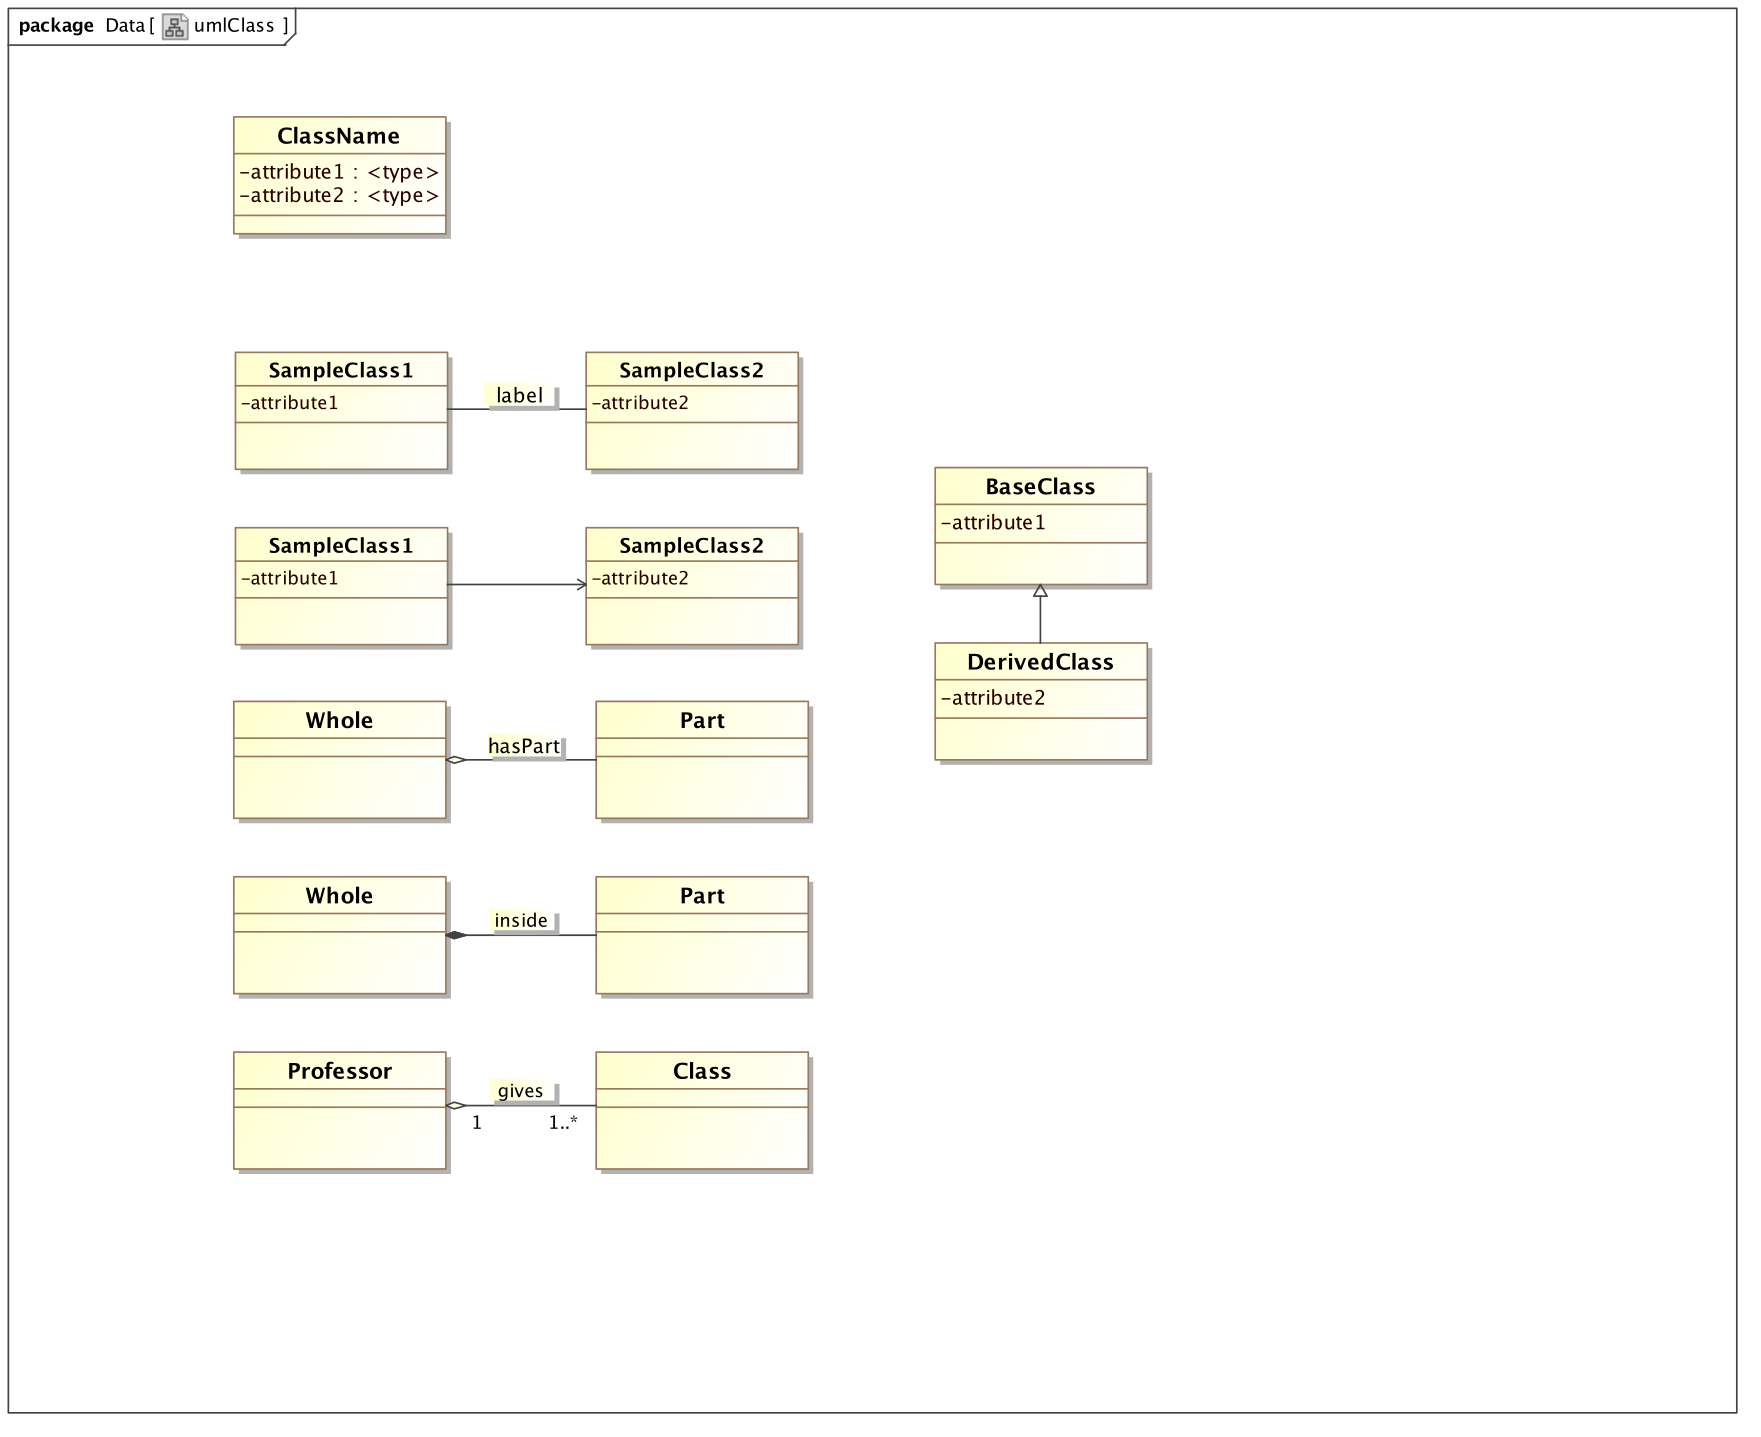
\includegraphics[width=0.2\textwidth]{images/uml/umlClass.png}
\caption{SED-ML UML Class with class names and attributes}
\label{fig:umlClass}
\end{figure}

SED-ML class names always begin with upper case letters. If they are composed of different words, the camel case style is used, as in e.\,g.\ \code{DataGenerator}.

\subsection{UML Relationships}
%% RELATIONS
\subsubsection{UML Relation Types}
\begin{figure}[h]
\centering
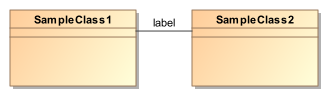
\includegraphics[width=0.5\textwidth]{images/uml/classRelation.png}
\caption{UML Class connectors}
\label{fig:umlConnectors}
\end{figure}

Links between classes specify the connection of objects with each other (\fig{umlConnectors}). The different relation types used in the SED-ML specification include aggregation, composite aggregation, and generalisation. The label on the line is called symbol (\code{label}) and describes the relation of the objects of both classes. 

%% Association
The \concept{association} (\fig{umlAssociation}) indicates the existence of a connection between the objects of the participating classes. Often associations are directed to show how the label should be read (in which direction). Associations can be uni-directional (one arrowhead), or bidirectional (zero or two arrowheads). 
\begin{figure}[h]
\centering
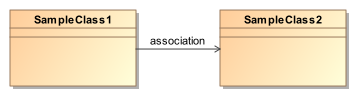
\includegraphics[width=0.5\textwidth]{images/uml/umlAssociation.png}
\caption{UML Association}
\label{fig:umlAssociation}
\end{figure}

 
%% Aggregation
The \concept{aggregation} (\fig{umlAggregation}, top) indicates that the objects of the participating classes are connected in a way that one class (\code{Whole}) consists of several parts (\code{Part}). In an aggregation, the parts may be independent of the whole. For example, a car (\code{Whole})  has several parts called wheel (\code{Part}); however, the wheels can exist independently of the car while the car requires the wheels in order to function.
\begin{figure}[h]
\centering
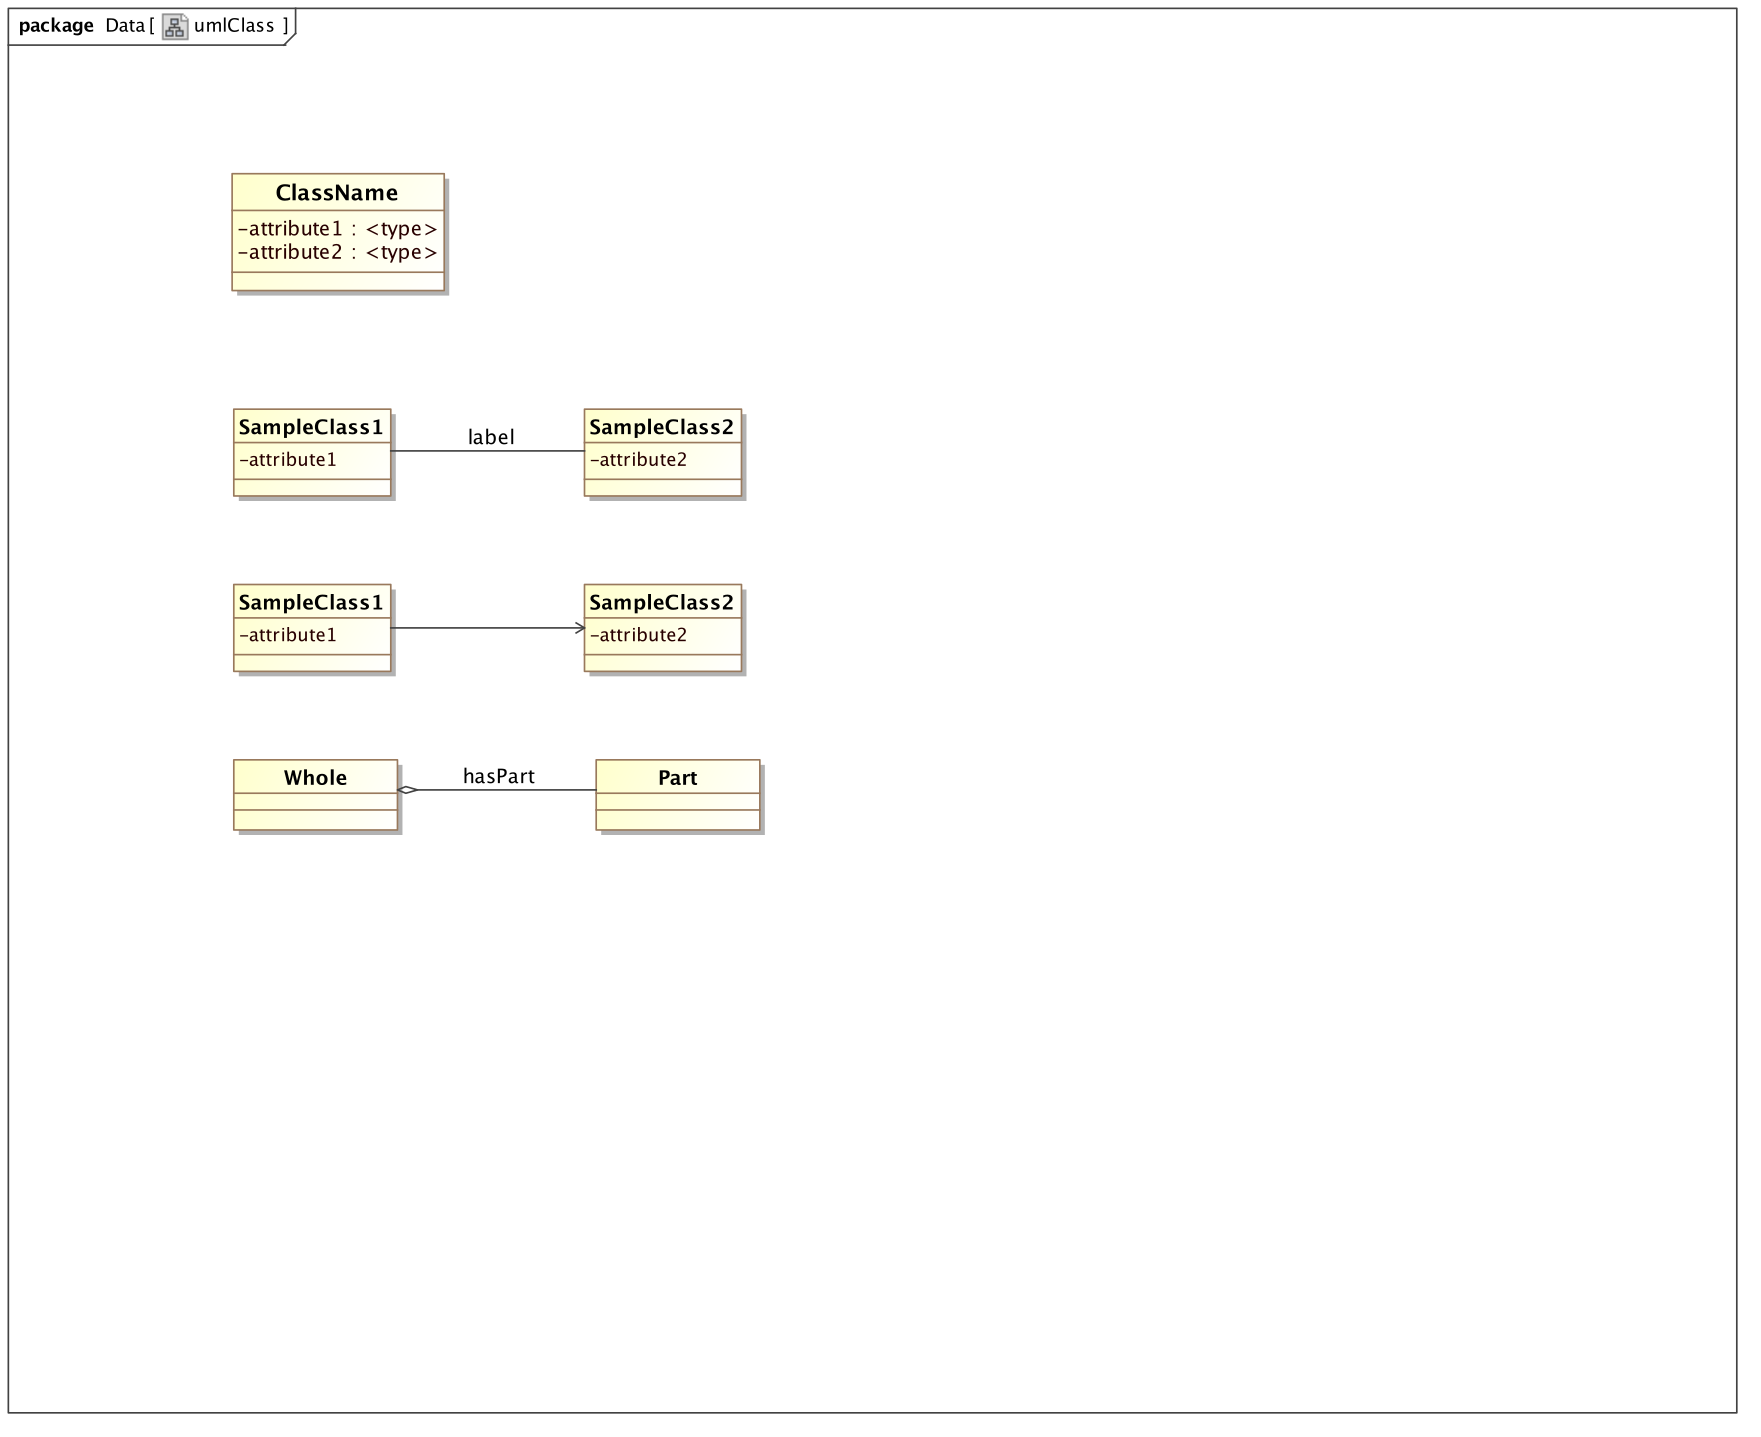
\includegraphics[width=0.5\textwidth]{images/uml/umlAggregation.png}
\caption{UML Aggregation}
\label{fig:umlAggregation}
\end{figure}

%% Composite Aggregation
The \concept{composite aggregation} (\fig{umlAggregation}, bottom) indicates that the objects of the participating classes are connected in a way that one class (\code{Whole}) consists of several parts (\code{Part}). In contrast to the aggregation, the subelements (\code{Part}) are dependent on the parent class (\code{Whole}). An example is that a university (\code{Whole}) consists of a number of departments (\code{Part}) which have a so-called ``lifetime responsibility'' with the university, e.\,g.\ if the university vanishes,  the departments will vanish with it \citep{Bel03}.

%% Inheritance
The \concept{generalisation} (\fig{umlGeneralisation}) allows to extend classes (\code{BaseClass}) by additional properties. The derived class (\code{DerivedClass}) inherites all properties of the base class and defines additional ones. In the given example, an instance of \code{DerivedClass} has two attributes \code{attribute1} and \code{attribute2}.
%
\begin{figure}[h]
\centering
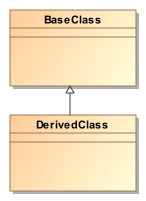
\includegraphics[width=0.2\textwidth]{images/uml/umlGeneralisation.png}
\caption{UML Generalisation}
\label{fig:umlGeneralisation}
\end{figure}
%
%% CARDINALITIES
\subsubsection{UML multiplicity}
UML multiplicity defines the number of objects in one class that can be related to one object in the other class (also known as \concept{cardinality}). Possible types of multiplicity include values (1), ranges (1$..$4), intervals (1,3,9), or combinations of ranges and intervals. The standard notation for ``many'' is the asterix (*). 

Multiplicity can be defined for both sides of a relationship between classes. The default relationship is ``many to many''. 
The example in \fig{umlMulti} expresses that a class is given by a professor, and a professor might give one to many classes.
\begin{figure}[h]
\centering
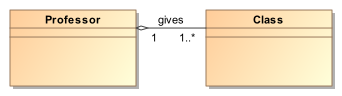
\includegraphics[width=0.4\textwidth]{images/uml/umlMultiplicity.png}
\caption{UML Multiplicity in an Aggregation}
\label{fig:umlMulti}
\end{figure}

%% XML SCHEMA
\subsection{XML Schema language elements}
The main building blocks of an XML Schema specification are:
\begin{itemize}
\item {simple and complex types}
\item {element specifications}
\item {attribute specifications}
\end{itemize}
XML Schema \concept{definitions} create new types, \concept{declarations} define new elements and attributes.
The definition of new (simple and complex) types can be based on a number of already existing, prefedined types (string, boolean, float). Simple types are restrictions or extensions of predefined types. Complex types describe how attribues can be assigned to elements and how elements can contain further elements. The current SED-ML XML Schema only makes use of \emph{complex type definitions}.
An example for a complex type definition is given in \lst{complexType}:
%
\begin{myXmlLst}{Complex Type definition of the SED-ML \code{computeChange} element}{lst:complexType}
<xs:element name="computeChange">
		<xs:complexType>
			<xs:complexContent>
				<xs:extension base="SEDBase">
					<xs:sequence>
						<xs:element ref="listOfVariables" minOccurs="0" />
						<xs:element ref="listOfParameters" minOccurs="0" />
						<xs:element ref="math" />
					</xs:sequence>
					<xs:attribute name="target" use="required" type="xs:token" />
				</xs:extension>
			</xs:complexContent>
		</xs:complexType>
	</xs:element>
\end{myXmlLst}
%
It shows the declaration of an element called \code{computeChange} that is used in SED-ML to change mathematical expressions. The element is defined using an \emph{unnamed} complex type which is build of further elements called \code{listOfVariables}, \code{listOfParameters}, and \code{math}. 
Additionally, the element \code{computeChange} has an attribute \code{target} declared. Please note that the definition of the elements inside the complex type are only referred to and will be found elsewhere in the schema.

The nesting of elements in the schema can be expressed using the \code{xs:sequence} (a sequence of elements), \code{xs:choice} (an alternative of elements to choose from), or \code{xs:all} (a set of elements that can occur in any order) concepts. The current SED-ML XML Schema only uses the \emph{sequence} of elements. 

\subsubsection{Multiplicities}
The standard multiplicity for each defined \code{element} is 1. Explicit multiplicity is to be defined using the \code{minOccurs} and \code{maxOccurs} attributes inside the complex type definition, as shown in \lst{multiplicity}.

\begin{myXmlLst}{Multiplicity for complex types in XML Schema}{lst:multiplicity}
<xs:element name="dataGenerator">
		<xs:complexType>
			<xs:complexContent>
				<xs:extension base="SEDBase">
					<xs:sequence>
						<xs:element ref="listOfVariables" minOccurs="0" />
						<xs:element ref="listOfParameters" minOccurs="0" />
						<xs:element ref="math" />
					</xs:sequence>
					<xs:attributeGroup ref="idGroup" />
				</xs:extension>
			</xs:complexContent>
		</xs:complexType>
	</xs:element>
\end{myXmlLst}
%
In this example, the \code{dataGenerator} type is build of a sequence of three elements: The \code{listOfVariables} element is not necessary for the definition of a valid \code{dataGenerator} XML structure (it may occur 0 times or once). The same is true for the \code{listOfParameters} element (it may as well occur 0 times or once). The \code{math} element, however, uses the implicit standard multiplicity -- it must occur exactly 1 time in the \code{dataGenerator} specification.

\subsection{Type extensions}
XML Schema offers mechanisms to restrict and extend previously defined complex types. Extensions add element or attribute declarations to existing types, while restrictions restrict the types by adding further characteristics and requirements (facets) to a type. An example for a type extension is given in \lst{xmlExtension}.
%
\begin{myXmlLst}{Definition of the sedML type through extension of SEDBase in SED-ML}{lst:xmlExtension}
	<xs:element name="sedML">
		<xs:complexType>
			<xs:complexContent>
				<xs:extension base="SEDBase">
					<xs:sequence>
						<xs:element ref="listOfSimulations" minOccurs="0" />
						<xs:element ref="listOfModels" minOccurs="0" />
						<xs:element ref="listOfTasks" minOccurs="0" />
						<xs:element ref="listOfDataGenerators" minOccurs="0" />
						<xs:element ref="listOfOutputs" minOccurs="0" />
					</xs:sequence>
					<xs:attribute name="level" type="xs:decimal" use="required"
						fixed="1" />
					<xs:attribute name="version" type="xs:decimal" use="required"
						fixed="1" />
				</xs:extension>
			</xs:complexContent>
		</xs:complexType>
	</xs:element>
\end{myXmlLst}
%
%% Q: How about renaming sedML to sed-ml for the next version?
The \code{sedML} element is an extension of the previously defined \code{SEDBase} type. It extends \code{SEDBase} by a sequence of five additional elements (\code{listOfSimulations}, \code{listOfModels}, \code{listOfTasks}, \code{listOfDataGenerators}, and \code{listOfOutputs}) and a new attribute \code{version}.

%% MAPPINGS
% \subsection{Mappings}

% \subsubsection{Mapping the Workflow Structure to a UML Class Diagram Structure}
% The main structure of the above shown workflow can be easily recognised in main class structure of the UML class diagram as shown in Figure \ref{fig:sedml}. Other processes of the workflow have been mapped to according class attributes and/or additional classes in the UML class diagram structure.

% \subsubsection{Conversion of UML into XML Schema}
% Also, the conversion of the UML class diagram representation into the XML Schema model is very intuitive and follows a small set of rules: UML Classes from the diagram are mapped to XML \alert{tbc}
% Page 6 of the SBML spec


%%% Local Variables: 
%%% mode: latex
%%% TeX-master: "../sed-ml-L1V2"
%%% End: 


%% CONCEPTS
\section{Concepts used in SED-ML}

  %% MATHML SUBSET USED
  % on the MathML subset used in SED-ML
\label{sec:mathML}
\subsection{The MathML Subset used in SED-ML}
The SED-ML specification allows for the pre-processing of computational models, 
as well as post processing of the simulation results. The corresponding 
mathematical expressions are encoded using MathML 2.0. MathML is an 
international standard for encoding mathematical expressions using XML and is 
used as representation of mathematical expressions in SBML and CellML, two of 
the languages supported by SED-ML. A problem arises, because the individual 
supported model exchange languages allow different subsets of MathML. Thus, 
when for example a ChangeXML element replaces a mathematical expression of  an 
SBML reaction, only the MathML subset allowed by SBML should be used here. 

In order to make the SED-ML format easier to adopt, at the beginning we 
restrict the MathML subset to the following operations: 

\begin{itemize}\setlength{\parskip}{-0.1ex}

\item \emph{token}: \token{cn}, \token{ci}, \token{csymbol},
  \token{sep}
  
\item \emph{general}: \token{apply}, \token{piecewise},
  \token{piece}, \token{otherwise}, \token{lambda} 

\item \emph{relational operators}: \token{eq}, \token{neq},
  \token{gt}, \token{lt}, \token{geq}, \token{leq}

\item \emph{arithmetic operators}: \token{plus}, \token{minus},
  \token{times}, \token{divide}, \token{power}, \token{root},
  \token{abs}, \token{exp}, \token{ln}, \token{log},
  \token{floor}, \token{ceiling}, \token{factorial}

\item \emph{logical operators}: \token{and}, \token{or},
  \token{xor}, \token{not}

\item \emph{qualifiers}: \token{degree}, \token{bvar},
  \token{logbase}

\item \emph{trigonometric operators}: \token{sin}, \token{cos},
  \token{tan}, \token{sec}, \token{csc}, \token{cot},
  \token{sinh}, \token{cosh}, \token{tanh}, \token{sech},
  \token{csch}, \token{coth}, \token{arcsin}, \token{arccos},
  \token{arctan}, \token{arcsec}, \token{arccsc}, \token{arccot},
  \token{arcsinh}, \token{arccosh}, \token{arctanh},
  \token{arcsech}, \token{arccsch}, \token{arccoth}

\item \emph{constants}: \token{true}, \token{false},
  \token{notanumber}, \token{pi}, \token{infinity},
  \token{exponentiale}

\item \emph{MathML annotations}: \token{semantics},
  \token{annotation}, \token{annotation-xml}

\end{itemize}

It should be noted, that all the operations listed above, only operate on 
singular values. However, as one of SED-ML's aim is to provide post processing 
on the results of simulation experiments, we need to enhance this basic set of 
operations by some aggregate functions. 

\subsubsection{Enabling post processing of simulation experiments}

The first step for enabling for post processing, is to define the symbols that 
represent vector values. To simplify things for SED-ML L1V1 the only symbols to 
be used are the identifiers of variables defined in the listOfVariables of 
DataGenerators. These variables represent the data collected from the 
simulation experiment with the associated task. 

To enable post processing the following aggregate functions are available for 
use with DataGenerator variables: 

\begin{itemize}\setlength{\parskip}{-0.1ex}

\item \emph{min}: Where the minimum of a variable represents the smallest value 
the simulation experiment yielded. Example: 

\begin{verbatim} <min> <ci> variableId </ci></min> \end{verbatim}.

\item \emph{max}: Where the maximum of a variables represents the largest value 
the simulation experiment yielded. Example: 

\begin{verbatim} <max> <ci> variableId </ci></max> \end{verbatim}.

\item \emph{sum}: All values of the variable returned by the simulation 
experiment are added up. Example: 

\begin{verbatim} <sum> <ci> variableId </ci></sum> \end{verbatim}.

\item \emph{product}: All values of the variable returned by the simulation 
experiment are multiplied. Example: 

\begin{verbatim} <product> <ci> variableId </ci></product> \end{verbatim}.

\end{itemize}

These represent the only exceptions. At this point SED-ML does not define a 
complete algebra of vector values. For more information see the description of 
DataGenerators.

%%% Local Variables: 
%%% mode: latex
%%% TeX-master: "../sed-ml-L1V1"
%%% End: 


  %% THE SUGGESTED URI SCHEME
  % The proposed URI scheme to use
  \subsection{URI Scheme}  
\label{sec:uriScheme}

URIs are needed at different points in SED-ML \LoneVtwo: 
Firstly, they are the preferred mechanism to refer to model encodings. 
Secondly, they are used to specify the language of the referenced model.
Thirdly, they enable addressing implicit model variables.
Finally, annotations of SED-ML elements should be provided with a standardised annotation scheme.

The use of a standardised URI Scheme ensures long-time availability  of particular information that can unambiguously be identified. 

\subsubsection{Model references}
\label{sec:modelURI}
The preferred way for referencing a model from a SED-ML file is adopted from the \concept{MIRIAM URI Scheme}.
MIRIAM enables identification of a data resource (in this case a model resource) by a predefined URN. A data entry inside that resource is identified by an ID. 
That way each single  model  in a particular model repository can be unambiguously referenced. To become part of MIRIAM resources, a model repository must ensure permanent and consistent model references, that is stable IDs.

One model repository that is part of MIRIAM resources is the \concept{BioModels Database} \citep{LDR+10}. Its data resource name in MIRIAM is \code{urn:miriam:biomodels.db}. To refer to a particular model, a standardised identifier scheme is defined in \concept{MIRIAM Resources}\footnote{\url{http://www.ebi.ac.uk/miriam/}}. The ID entry maps to a particular model in the model repository. That model is never deleted. 
A sample BioModels Database ID is \code{BIOMD0000000048}. Together with the data resource name it becomes unambiguously identifiable by the URN \code{urn:miriam:biomodels.db:BIOMD0000000048} (in this case referring to the 1999 Kholodenko model on EGFR signaling). 
%

SED-ML recommends to follow the above scheme for model references, if possible. 
SED-ML does not specify how to resolve the URNs. However, MIRIAM Resources offers web services to do so\footnote{\url{http://www.ebi.ac.uk/miriam/}}. For the above example of the \code{urn:miriam:biomodels.db:BIOMD0000000048} model, the resolved URL may look like: 
\begin{itemize}
 \item{\code{http://biomodels.caltech.edu/BIOMD0000000048} or}
 \item{\code{http://www.ebi.ac.uk/biomodels-main/BIOMD0000000048}}
\end{itemize}
depending on the physical location of the resource chosen to resolve the URN.

An alternative means to obtain a model may be to provide a single resource containing necessary models and a SED-ML file. Although a specification of such a resource is beyond the scope of this document,  one proposal  --  SED-ML archive format -- is  described   in Appendix~\ref{app:archive}.
Further information on the \hyperref[sec:source]{source} attribute referencing the model location is provided in Section~\ref{sec:source}.

\subsubsection{Language references}
\label{sec:languageURI}
To specify the language a model is encoded in, a set of pre-defined SED-ML URNs can be used. 
The structure of SED-ML language URNs is \element{urn:sedml:language:}\emph{name.version}. 
SED-ML allows to specify a model representation format very generally as being \code{XML}, if no standardised representation format has been used to encode the model. On the other hand, one can be as specific as defining
a model being in a particular version of a language, as ``SBML Level 2, Version 2, Revision 1''.

The list of URNs is available from \url{http://sed-ml.org/}. 
Further information on the \hyperref[sec:language]{language} attribute is provided in Section~\ref{sec:language}.

\subsubsection{Implicit variables}
\label{sec:implicitVariable}

Some variables used in an experiment are not explicitly defined in the model, but may be implicitly contained in it. 
For example, to plot a variable's behaviour over time, that variable is defined in an SBML model, while \emph{time} is not explicitly defined. 

To overcome this issue and allow SED-ML to refer to such variables in a common way, the notion of \emph{implicit variables} is used.
Those variables are called \code{symbols} in SED-ML. They are defined following the idea of MIRIAM URNs and using the SED-ML URN scheme. The structure of the URNs is \element{urn:sedml:symbol:}\emph{implicit variable}.
To refer from a SED-ML file to the definition of \emph{time}, for example, the URN is \element{urn:sedml:symbol:time}.

The list of predefined symbols is available from the SED-ML site on \url{http://sed-ml.org/}.
From that source, a mapping of SED-ML symbols on possibly existing concepts in the single languages supported by SED-ML is provided.

\subsubsection{Annotations}
\label{sec:annotations}
When annotating SED-ML elements with semantic \hyperref[class:annotation]{annotation}s, the \concept{MIRIAM URI Scheme} should be used. In addition to providing the data type (e.\,g.\ PubMed) and the particular data entry inside that data type (e.\,g.\ \code{10415827}), the relation of the annotation to the annotated element should be described using the standardised \concept{biomodels.net qualifier}. The list of qualifiers, as well as further information about their usage, is available from \url{http://www.biomodels.net/qualifiers/}.


%%% Local Variables: 
%%% mode: latex
%%% TeX-master: "../sed-ml-L1V1"
%%% End: 

  
  %%XPATH
  % XPath
\subsection{XPath usage}  

\label{sec:xpath} 
XPath is a language for finding information in an XML document \citep{xpath:1999}. Within \LoneVone, XPath version 1 expressions are  used to identify nodes and attributes within an XML representation of a biological model in the following ways:
%
\begin{enumerate}
\item {Within a \hyperref[class:variable]{Variable} definition, where XPath identifies the model variable required for manipulation in SED-ML.}
\item {Within a  \hyperref[class:change]{Change} definition, where XPath is used to identify the target XML to which a change should be applied.} 

\end{enumerate}

For proper application, XPath expressions should contain prefixes that allow their resolution to the correct XML namespace within an XML document. For example, the XPath expression referring to a species \emph{X} in an SBML model:
\begin{alltt}
/sbml:sbml/sbml:model/sbml:listOfSpecies/sbml:species[@id=`X'] {\color{green} \tickYes -\emph{CORRECT}}
\end{alltt}
is preferable to 
\begin{alltt}
/sbml/model/listOfSpecies/species[@id=`X'] {\color{red} \tickNo -\emph{INCORRECT} }
\end{alltt}

which will only be interpretable by standard XML software tools  if the SBML file declares no namespaces. 




%%% Local Variables: 
%%% mode: latex
%%% TeX-master: "../sed-ml-L1V1"
%%% End: 

  
  %% KISAO
  % KiSAO
\label{sec:kisao}

An important aspect of a simulation experiment is the simulation algorithm used to solve the system.

The sole reference of a simulation algorithm through its name in form of a string is error prone and unambiguous. Firstly, typing mistakes or language differences may make the identification of the intended algorithm difficult. Secondly, many algorithms exist with more than one name, having synonyms or various abbriviations that are commonly used.

These problems can be solved by using controlled vocabulary to refer to a particular simulation algorithm. One attempt to provide such a vocabulary is the \emph{Kinetic Simulation Algorithm Ontology} (KiSAO, \url{http://www.ebi.ac.uk/compneur-srv/kisao/}). KiSAO is a community-driven approach of classifying and structuring simulation approaches by model characteristics and numerical characteristics.  Model characteristics include, for instance, the type of variables used for the simulation (such as discrete or continuous variables) and the spatial resolution (spatial or non-spatial descriptions). Numerical characteristics specify whether the system's behavior can be described as deterministic or stochastic, and whether the algorithms use fixed or adaptive time steps.  
Related algorithms are grouped together, producing classes of algorithms \citep{CWK+10}.

Although work is still at an early stage, the use of KiSAO is recommended when referring to a simulation algorithm from a SED-ML description. The use of KiSAO for the moment is limited to looking up the algorithm that was used in the simulation experiment (through resolving the KiSAO ID) and then to try and use one algorithm that is as similar to the original one as possible. KiSAO will become more supportive for SED-ML as soon as the ontology contains a wider range of relationships between different algorithms, as well as extended descriptions of the algorithm characteristics.


%%% Local Variables: 
%%% mode: latex
%%% TeX-master: "../sed-ml-L1V1"
%%% End: 




% ~~~~~~~~~~~~~~~~~~~~~~~~~~~~~~~~~~~~
%% RESOURCES
% ~~~~~~~~~~~~~~~~~~~~~~~~~~~~~~~~~~~~
 \subsection{SED-ML resources}
% further resources
%Further information on SED-ML as well as an extensive example for a SED-ML file can be be found in ``SED-ML -- An XML Format for the Implementation of the MIASE Guidelines'' \citep{KL08a}.
% -> I removed the reference to the CMSB paper, as the UML is slightly different to the one presented there. To avoid confusion.

SED-ML is part of the biomodels.net initiative \url{http://www.biomodels.net}. Information on SED-ML can be found on \url{http://www.biomodels.net/sed-ml}.

The SED-ML XML Schema, the UML schema and related implementations, libraries, validators and so on can be found on the SED-ML sourceforge project page \url{http://sed-ml.svn.sourceforge.net/}.



%%% Local Variables: 
%%% mode: latex
%%% TeX-master: "../sed-ml-L1V1"
%%% End: 




% ~~~~~~~~~~~~~~~~~~~~~~~~~~~~~~~~~~~~
%% GENERAL LANGUAGE ELEMENTS
% ~~~~~~~~~~~~~~~~~~~~~~~~~~~~~~~~~~~~
  \section{General attributes and classes}
In this section we introduce attributes and concepts used repeatedly throughout the SED-ML specification. 

\subsection{The \element{xmlns} attribute}
\label{sec:xmlns}
The \concept{xmlns} attribute contains namespace declarations for elements of external languages used in SED-ML.

First of all, \code{xmlns} declares the namespace for the SED-ML document. The pre-defined standard namespace is \url{http://www.biomodels.net/sed-ml}. 

In addition, SED-ML makes use of the \concept{MathML} namespace \url{http://www.w3.org/1998/Math/MathML} to enable the encoding of mathematical expressions in MathML 2.0. SED-ML uses a subset of MathML as described in section \ref{sec:mathML} on page \pageref{sec:mathML}.

SED-ML \concept{notes} use the \code{xmlns} of XHTML \url{http://www.w3.org/1999/xhtml}.  The \hyperref[class:notes]{Notes} class is described in section \ref{class:notes} on page \pageref{class:notes}.

%All namespace declarations will be omitted in the following SED-ML sample code snippets.

%%% Local Variables: 
%%% mode: latex
%%% TeX-master: "../sed-ml-L1V1"
%%% End: 


\subsection{The \element{id}  attribute}
\subsection{\element{id}}
\label{sec:id}
%

Most objects in SED-ML carry an \concept{id} attribute. 
The \hyperref[sec:id]{id} attribute, if it exists for an object, is always required and identifies SED-ML constituents unambiguously.   
The data type for \code{id} is \code{SId} which is a datatype derived from the basic XML type \code{string}, but with restrictions about the characters permitted and the sequences in which those characters may appear. The definition is shown in
Figure~\vref{fig:sid}.

\begin{figure}[hbt]
  \ttfamily
  \small
  \centering
  \begin{tabular}{lll}
    letter & ::= & 'a'..'z','A'..'Z'\\
    digit  & ::= & '0'..'9'\\
    idChar & ::= & letter | digit | '\_'\\
    SId    & ::= & ( letter | '\_' ) idChar*\\
  \end{tabular}
  \vspace*{-1ex}
  \caption{The definition of the type \code{SId}}
  \label{fig:sid}
\end{figure}

For a detailed description see also the SBML specification on the ``Type SId'' \citep[p. 11]{HBH+10}.

All \code{id}s have a global scope, i.\,e.\ the \code{id} must be unambiguous throughout a whole SED-ML document. As such it identifies the constituent it is related to.

An example for a defined \concept{id} is given in Listing~\ref{lst:id}.
%
\begin{myXmlLst}{SED-ML identifier definition, e.\,g.\ for a model}{lst:id}
<model id="m00001" language="urn:sedml:language:sbml" source="urn:miriam:biomodels.db:BIOMD0000000012">
 [MODEL DEFINITION]
</model>
\end{myXmlLst}
%
The defined model carries the  \code{id} \code{m00001}. If the model is referenced elsewhere in the SED-ML document, it is referred to by that  \code{id}.

%%% Local Variables: 
%%% mode: latex
%%% TeX-master: "../sed-ml-L1V2"
%%% End: 


\subsection{The \element{name} attribute}
\subsection{\element{name}}
\label{sec:name}
%

Besides an \hyperref[sec:id]{id}, a SED-ML constituent may carry an optional \concept{name}. However, names do not have identifying character;  several SED-ML constituents may carry the same name. The purpose of the \code{name} attribute is to keep a human-readable name of the constituent, e.\,g.\ for display to the user. In the XML Schema representation, names are of the data type \code{String}.

Listing \ref{lst:name} extends the model definition in \lst{id} by a model name.
%
\begin{myXmlLst}{SED-ML name definition, e.\,g.\ for a model}{lst:name}
<model id="m00001" name="Circadian oscillator" language="urn:sedml:language:sbml" source="urn:miriam:biomodels.db:BIOMD0000000012">
 [MODEL DEFINITION]
</model>
\end{myXmlLst}
%

%%% Local Variables: 
%%% mode: latex
%%% TeX-master: "../sed-ml-L1V3"
%%% End: 

\newpage
\subsection{The SEDBase Class}
% SED-Base class
\subsection{\element{SEDBase}}
\label{class:sedBase}
\concept{SEDBase} is the base class  of SED-ML \currentLV. All other classes are derived from it. As such it provides means to attach additional information on all other classes  (\fig{sedBase}). That information can be specified by human readable \hyperref[class:notes]{Notes} or custom \hyperref[class:annotation]{Annotations}. 
%
\sedfig[width=0.9\textwidth]{pdf/sedBaseClass}{The SEDBase class}{fig:sedBase}
%

%SEDBase has one optional attribute \hyperref[sec:metaID]{metaID}. 

\tabtext{sedbase}{SEDBase}
%
\begin{table}[ht]
\center
\begin{tabular}{|l|l|}
\hline
\textbf{\attribute} & \textbf{\desc}\\
\hline
metaid$^{o}$ & \refpage{sec:metaID} \\
\hline
\hline
\textbf{\subelements} & \textbf{\desc}\\
\hline
notes$^{o}$ & \refpage{class:notes}\\
annotation$^{o}$ & \refpage{class:annotation}\\
\hline
\end{tabular}
\caption{\tabcap{SEDBase}}
\label{tab:sedbase}
\end{table}
%

\input{sources/metaid}

\input{sources/notesClass}

\input{sources/annotationClass}


%%% Local Variables: 
%%% mode: latex
%%% TeX-master: "../sed-ml-L1V3"
%%% End: 


\subsubsection{The Notes Class}
\label{class:notes}

A \concept{note} is considered a  human-readable description of the element it is assigned to. It serves to display information to the user. 
Instances of the \concept{Notes} class may contain any valid XHTML \citep{P+02}, ranging from short comments to whole HTML pages for display in a Web browser. 
The namespace URL for \code{XHTML} content inside the \hyperref[class:notes]{Notes} class is \url{http://www.w3.org/1999/xhtml}. It may either be declared in the \hyperref[class:sed-ml]{\code{sedML} XML element}, or directly for use in each \code{notes} element of the XML file. For further options of how to set the namespace and detailed examples, please refer to (\citep{HBH+10}, p. 14).

\tabtext{notes}{notes}
%
\begin{table}[ht]
\center
\begin{tabular}{|l|l|}
\hline
\textbf{\attribute} & \textbf{\desc}\\
\hline
xmlns & \refpage{sec:xmlns} \\
\hline
\hline
\textbf{\subelements} & \textbf{\desc}\\
\hline
\emph{none} & \\
\hline
\end{tabular}
\label{tab:notes}
\caption{\tabcap{Notes}}
\end{table}
%
\code{Notes} has a mandatory attribute \hyperref[sec:xmlns]{xmlns} to declare the \code{XHTML} namespace. It does not have any further sub-elements nor attributes associated to it.
%

\lsttext{notes}{notes}
%
\begin{myXmlLst}{The \element{notes} element}{lst:notes}
<sedML [..]>
 <notes http://www.w3.org/1999/xhtml>
  The enclosed simulation description shows the oscillating behaviour of the Repressilator model using deterministic and stochastic simulators.
 </notes>
</sedML>
\end{myXmlLst}
%
In this example, the namespace declaration is inside the \element{notes} element and the note is related to the \element{sedML} root element of the SED-ML file. A note may, however, occur inside \emph{any} SED-ML XML element, except \code{note} itself and \hyperref[class:annotation]{\code{annotation}}.

%%% Local Variables: 
%%% mode: latex
%%% TeX-master: "../sed-ml-L1V1"
%%% End: 


\subsubsection{The Annotation Class}
\label{class:annotation}

An \concept{annotation} is considered a computer-processible piece of information.
Annotations may contain any valid XML content. 
%No additional namespace declaration is needed for use of the annotation element. However, for the type of XML inside annotation, the according namespaces should be declared, if necessary.
For further guidelines on how to use annotations, we would like to encourage the reading of the corresponding section in the SBML specification \citep[pp. 14-16]{HBH+10}. The style of annotations in SED-ML is briefly described in section \ref{sec:annotations} on page \pageref{sec:annotations}.

%\concept{Annotation} does not define any further attributes, nor does it have classes associated to it. 

\tabtext{annotation}{Annotation}
%
\begin{table}[ht]
\center
\begin{tabular}{|l|l|}
\hline
\textbf{\attribute} & \textbf{\desc}\\
\hline
\emph{none} & \\
\hline
\hline
\textbf{\subelements} & \textbf{\desc}\\
\hline
\emph{none in the SED-ML namespace} & \\
\hline
\end{tabular}
\label{tab:annotation}
\caption{\tabcap{Annotation}}
\end{table}
%

\lsttext{annotation}{annotation}
%
\begin{myXmlLst}{The annotation element}{lst:annotation}
<sedML>
  [..]
  <model id="model1" metaID="001" language="urn:sedml:language:cellml" 
   source="http://models.cellml.org/workspace/leloup_gonze_goldbeter_1999/@@rawfile/d6613d7e1051b3eff2bb1d3d419a445bb8c754ad/leloup_gonze_goldbeter_1999_a.cellml" >
   <annotation>
    <rdf:RDF xmlns:rdf="http://www.w3.org/1999/02/22-rdf-syntax-ns#" 
             xmlns:bqmodel="http://biomodels.net/model-qualifiers/">
     <rdf:Description rdf:about="#001">
      <bqmodel:isDescribedBy>
       <rdf:Bag>
        <rdf:li rdf:resource="urn:miriam:pubmed:10415827"/>
       </rdf:Bag>
      </bqmodel:isDescribedBy>
     </rdf:Description>
    </rdf:RDF>
   </annotation>
  </model>
  [..]
</sedML>
\end{myXmlLst}
%
In that example, a SED-ML \hyperref[class:model]{model} element is annotated with a reference to the original publication. The \element{model} contains an \element{annotation} that uses the \concept{biomodels.net model-qualifier} \element{isDescribedBy} to link to the external resource \element{urn:miriam:pubmed:10415827}. 
In natural language the annotation content could be interpreted as ``The model \emph{is described by} the published article available from \emph{pubmed} under ID \emph{10643740}''. 
The example annotation follows the proposed \hyperref[sec:uriScheme]{URI Scheme} suggested by the MIRIAM reference standard. The MIRIAM URN can be resolved to the PubMED (\url{http://pubmed.gov}) publication with ID 10415827, namely the article ``Alternating oscillations and chaos in a model of two coupled biochemical oscillators driving successive phases of the cell cycle.'' published by Romond et al. in  1999.   


%%% Local Variables: 
%%% mode: latex
%%% TeX-master: "../sed-ml-L1V1"
%%% End: 


\newpage
\subsection{The SED-ML Class}
% sed-ml Class
\subsection{\element{SED-ML} top level element}
\label{class:sed-ml}
Each SED-ML \LoneVone document has a main class called SED-ML which defines the document's structure and content (\fig{sed-mlMain}).
%
%\sedfig[width=0.35\textwidth]{sed-mlClass}{The SED-ML class}{fig:sed-ml}
%
It consists of several parts; the parts are all connected to the SED-ML class through aggregation: 
the \hyperref[class:model]{Model} class (for model specification, see Section~\ref{class:model}), the \hyperref[class:simulation]{Simulation} class (for simulation setup specification, see Section~\ref{class:simulation}), the \hyperref[class:task]{Task} class (for the linkage of models and simulation setups, see Section~\ref{class:task}), the \hyperref[class:dataGenerator]{DataGenerator} class (for the definition of post-processing, see Section~\ref{class:dataGenerator}), and the \hyperref[class:output]{Output} class (for the output specification, see Section~\ref{class:output}). All of them are shown in \fig{sed-mlMain} and will be explained in more detail in the relevant sections of this document.
%
\sedfig[width=0.8\textwidth]{sed-mlMain}{The sub-classes of SED-ML}{fig:sed-mlMain}
%

\tabtext{sed-ml}{SED-ML}

%
\begin{table}[ht]
\center
\begin{tabular}{|l|l|}
\hline
\textbf{\attribute} & \textbf{\desc}\\
\hline
metaID$^{o}$ & \refpage{sec:metaID}\\
xmlns & \refpage{sec:xmlns}\\
level & \refpage{sec:level}\\
version & \refpage{sec:version}\\
\hline
\hline
\textbf{\subelements} & \textbf{\desc}\\
\hline
notes$^{o}$ & \refpage{class:notes}\\
annotation$^{o}$ & \refpage{class:annotation}\\
listOfModels$^{o}$ & \refpage{sec:listOfModels}\\
listOfSimulations$^{o}$ & \refpage{sec:listOfSimulations} \\
listOfTasks$^{o}$ & \refpage{sec:listOfTasks} \\
listOfDataGenerators$^{o}$ & \refpage{sec:listOfDataGenerators} \\
listOfOutputs$^{o}$ & \refpage{sec:listOfOutputs} \\
\hline
\end{tabular}
\caption{\tabcap{SED-ML}}
\label{tab:sed-ml}
\end{table}
%
A SED-ML document needs to have the SED-ML namespace defined through the mandatory \hyperref[sec:xmlns]{xmlns} attribute. In addition, the SED-ML \hyperref[sec:level]{level} and \hyperref[sec:version]{version} attributes are mandatory.

The basic XML structure of a SED-ML file is shown in listing  \vref{lst:sedmlRoot}.
%
\begin{myXmlLst}{The SED-ML root element}{lst:sedmlRoot}
<?xml version="1.0" encoding="utf-8"?>
<sedML xmlns:math="http://www.w3.org/1998/Math/MathML" 
       xmlns="http://sed-ml.org/" level="1" version="1">
 <listOfModels />
  [MODEL REFERENCES AND APPLIED CHANGES]
 <listOfSimulations />
  [SIMULATION SETUPS]
 <listOfTasks />
  [MODELS LINKED TO SIMULATIONS]
 <listOfDataGenerators />
  [DEFINITION OF POST-PROCESSING]
 <listOfOutputs />
  [DEFINITION OF OUTPUT]
</sedML>
\end{myXmlLst}
%
The root element of each SED-ML XML file is the \code{sedML} element, encoding \hyperref[sec:version]{version} and \hyperref[sec:level]{level} of the file, and setting the necessary namespaces. Nested inside the \code{sedML} element are the five lists serving as containers for the encoded data (\concept{listOfModels} for all models, \concept{listOfSimulations} for all simulations, \concept{listOfTasks} for all tasks, \concept{listOfDataGenerators} for all post-processing definitions, and \concept{listOfOutputs} for all output definitions).

\input{sources/xmlns}

\input{sources/level}

\input{sources/version}


%%% Local Variables: 
%%% mode: latex
%%% TeX-master: "../sed-ml-L1V1"
%%% End: 


\newpage
\subsection{The reference Relations}
\label{sec:reference}

The \concept{reference} concept is used to refer to a particular element inside the SED-ML document. It may occur in four different ways in the SED-ML document:
\begin{enumerate}
\item{as an association between a \hyperref[class:variable]{Variable} and a \hyperref[class:model]{Model} (\hyperref[sec:modelReference]{modelReference})}
\item{as an association between a \hyperref[class:variable]{Variable} and a \hyperref[class:task]{Task} (\hyperref[sec:taskReference]{taskReference})}
\item{as an association between a \hyperref[class:task]{Task} and the associated \hyperref[class:model]{Model} (\hyperref[sec:modelReference]{modelRereference}) or}
\item{as an association between a \hyperref[class:task]{Task} and the \hyperref[class:simulation]{Simulation} (\hyperref[sec:simulationReference]{simulationReference})}
\end{enumerate}

Depending on the use of the \concept{reference} relation in connection with a \hyperref[class:variable]{Variable} object, it may take different roles: 
\begin{enumerate}
\item[a.]{The \concept{reference} association might occur between a Variable object and a Model object, if the variable is to define a \hyperref[class:change]{Change}. 
In that case the \code{variable} element contains a \hyperref[sec:modelReference]{modelReference} to refer to the particular model that contains the variable used to define the change (see section \ref{sec:modelReference} on page \pageref{sec:modelReference}). }
\item[b.]{If the \concept{reference} is used as an association between a Variable object and a Task object  inside the \hyperref[class:dataGenerator]{dataGenerator} class, then the \code{variable} element contains a \hyperref[sec:taskReference]{taskReference} to unambiguously refer to an observable in a given task (see section \ref{sec:taskReference} on page \pageref{sec:taskReference}).}
\end{enumerate}

The definition of a \hyperref[class:task]{Task} object demands a reference to a particular Model object (\hyperref[sec:modelReference]{modelReference}, see \ref{sec:modelReference} on page \pageref{sec:modelReference}); furthermore, the Task object must be associated with a particular Simulation object (\hyperref[sec:simulationReference]{simulationReference}, see \ref{sec:simulationReference} on page \pageref{sec:simulationReference}).


\subsubsection{model Reference}
\label{sec:modelReference}
%
The \concept{modelReference} represents a relation between a \hyperref[class:variable]{Variable} object and a \hyperref[class:Model]{Model} object, or  a relation between a \hyperref[class:Task]{Task} object and a \hyperref[class:Model]{Model} object.

If pre-processing needs to be applied to a model before simulation, then the model update can be specified by creating a \hyperref[class:Change]{Change} object. In the particular case that a change must be calculated with a mathematical function, variables need to be defined. To refer to an existing entity in a defined \hyperref[class:model]{Model}, the \concept{modelReference} is used. 

The \code{modelReference} attribute of the \code{variable} element contains a \concept{modelID}.
\lsttext{modelReference1}{modelReference} 
%
\begin{myXmlLst}{SED-ML \code{modelReference} attribute inside a variable definition of a  \code{computeChange} element}{lst:modelReference1}
<model id="m0001" [..]>
 <listOfChanges>
   <computeChange>
    <listOfVariables>
     <variable id="v1" modelReference="cellML" target="/cellml:model/cellml:component[@cmeta:id='MP']/cellml:variable[@name='vsP']/@initial_value" />
    </listOfVariables>
    <listOfParameters [..] />
    <math>
     [CALCULATION OF CHANGE]
    </math>
   </computeChange>
 </listOfChanges>
 [..]
</model>
\end{myXmlLst}
%
In the example, a change is  applied on model \code{m0001}. In the \code{computeChange} a list of variables is defined. One of those variable is \code{v1} which is defined in another model, namely \code{cellML}. To identify the variable in model \code{cellML} the XPath expression given in the \hyperref[sec:target]{target} attribute.

The \concept{modelReference} is as well used to define that a \hyperref[class:model]{Model} object is used in a particular  \hyperref[class:task]{Task}. Listing \ref{lst:modelReference2} shows how this can be done for a sample SED-ML document.
%
\begin{myXmlLst}{SED-ML \code{modelReference} definition inside a \element{task} element}{lst:modelReference2}
<listOfTasks>
 <task id="t1" name="Baseline" modelReference="model1" simulationReference="simulation1" />
 <task id="t2" name="Modified" modelReference="model2" simulationReference="simulation1" />
</listOfTasks>
\end{myXmlLst}
%
The example defines two different tasks, the first one applies the simulation settings of \code{simulation1} on \code{model1}, the second one applies the same simulation settings on \code{model2}.

\subsubsection{taskReference}
\label{sec:taskReference}
\hyperref[class:dataGenerator]{DataGenerator} objects are created to apply post-processing to the simulation results before simulation output. 

For certain types of post-processing \hyperref[class:variable]{Variable} objects need to be created. Those link to a defined \hyperref[class:task]{Task} from which the model that contains the variable of interest can be inferred. 
A \concept{taskReference} association is used to realise that link from a \hyperref[class:variable]{Variable} object inside a \hyperref[class:dataGenerator]{DataGenerator} to a \hyperref[class:task]{Task} object. 
Listing \ref{lst:reference3} gives an example.
%
\begin{myXmlLst}{SED-ML \code{taskReference} definition inside a \element{dataGenerator} element}{lst:reference3}
<listOfDataGenerators>
 <dataGenerator id="tim3" name="tim mRNA (difference v1-v2+20)">
  <listOfVariables>
   <variable id="v1" taskReference="t1" [..] />
  </listOfVariables>
  <math />
 </dataGenerator>
</listOfDataGenerators>
\end{myXmlLst}
%
The example shows the definition of a variable \code{v1} in a \code{dataGenerator} element. The variable appears in the model that is used in task \code{t1}. The task definition of \code{t1} might look as follows:
\begin{myXmlLst}{}{}
<listOfTasks>
  <task id="t1" name="task definition" modelReference="model1" 
        simulationReference="simulation1" />
</listOfTasks>
\end{myXmlLst}
Task \code{t1} references the model \code{model1}. Therefore we can conclude that the variable \code{v1} defined in listing \ref{lst:reference3} targets an element of the model with ID \code{model1}. The targeting process itself will be explained in section \ref{sec:target} on \refpage{sec:target}.

\subsubsection{simulationReference}
\label{sec:simulationReference}
The \concept{simulationReference} is used to refer to a particular \hyperref[class:simulation]{Simulation} in a \hyperref[class:task]{Task}. 
Listing \ref{lst:modelReference2}  on \refpage{lst:modelReference2} shows how the reference to a defined simulation for a sample SED-ML document. In the example, both tasks \code{t1} and \code{t2} use the simulation settings defined in \code{simulation1} to run the experiment.
%%% Local Variables: 
%%% mode: latex
%%% TeX-master: "../sed-ml-L1V1"
%%% End: 

\newpage
\subsection{The Variable Class}
% variable class
\label{class:variable}
Variables in SED-ML are references to already existing constituents in one of the defined \hyperref[class:model]{models}. A variable always is placed inside a \hyperref[class:listOfVariables]{listOfVariables}.
%
\sedfig[width=0.35\textwidth]{variableClass}{The Variable class}{fig:variable}
%
Each instance of the \concept{Variable} class  (see \fig{variable}) has a required \hyperref[sec:id]{id} and an optional \hyperref[sec:name]{name}. 
Variables are used to either refer to a model constituent, i.\,e. a model observable, such as an SBML species, or to refer to am implicit variable. 
The referenced constituent is specified through the mandatory \hyperref[sec:target]{target} attribute in the first case, and through a \hyperref[sec:symbol]{symbol} holding a MIRIAM URI in the second case. 

Listing \ref{lst:variable} shows a model with a listOfVariables declared that holds the variable definitions.
%
\begin{myXmlLst}{SED-ML \code{variable} definition}{lst:variable}
<model [..]>
 <listOfVariables>
   [VARIABLE DEFINITIONS FOLLOWING]
 </listOfVariables>
 [..]
</model>
\end{myXmlLst}
%

\tabtext{variable}{Variable}
%
\begin{table}[ht]
\center
\begin{tabular}{|l|l|}
\hline
\textbf{\attribute} & \textbf{\desc}\\
\hline
metaid$^{o}$ & \refpage{sec:metaID}\\
id & \refpage{sec:id} \\
name$^{o}$ & \refpage{sec:name}\\
\hline
target & \refpage{sec:target}\\
symbol & \refpage{sec:symbol}\\
\hline
taskReference & \refpage{sec:taskReference}\\
modelReference & \refpage{sec:modelReference}\\
\hline
\hline
\textbf{\subelements} & \textbf{\desc}\\
\hline
notes$^{o}$ & \refpage{class:notes}\\
annotation$^{o}$ & \refpage{class:annotation}\\
\hline
\end{tabular}
\label{tab:variable}
\caption{\tabcap{Variable}}
\end{table}

The \hyperref[sec:reference]{reference} to an object of the \concept{Variable} class may occur in two different places of the SED-ML document: 

First, it may occur in the \hyperref[class:change]{Change} class where it is used for describing the mathematical computation of a change of a model's observable, using other observables existing in a defined \hyperref[class:model]{model}.

The second use of the \concept{Variable} class is for defining a \hyperref[class:dataGenerator]{DataGenerator}. Here, a variable in an existing model or an implicit variable might be used to define the post-processing of the simulation.

\subsubsection{The \element{target} attribute}
\label{sec:target}
An instance of \concept{Variable} refers to a model constituent inside a particular \hyperref[class:model]{model} through an \concept{XPath} expression stored in the required \concept{target} attribute. 

XPath allows to unambiguously identify an element or attribute in an XML file.

An example for a variable definition is given in listing \ref{lst:variable}.
%
\begin{myXmlLst}{SED-ML \code{target} definition}{lst:target}
<model id="m0001" language="urn:sedml:language:sbml" source="urn:miriam:biomodels.db:BIOMD0000000012">
 <listOfChanges>
  <computeChange>
   <listOfVariables>
    <variable id="v1" name="Tet Repressor protein" taskreference="t1"  target="/sbml/listOfSpecies/species[@id="PY"]" />
   </listOfVariables>
   [CHANGE DEFINITION FOLLOWING]
  </computeChange>
 </listOfChanges>
</model>
\end{myXmlLst}
%
Please note that the identifier and names inside the SED-ML document do not have to comply with the identifiers and names that the model and its constituents carry in the model definition. In the above example \ref{lst:variable}, the variable with ID \code{v1} is defined. It is described as the \code{TetR protein}. The reference points to a species in the referenced SBML model. The particular species can be identified through its ID in the SBML model, namely \code{PY}. However, SED-ML does not forbid to use identical identifiers and names as in the referenced models neither. The following is the same valid SED-ML example for the specification of a variable as the above in listing \ref{lst:variable}, but with different naming:
%
\begin{myXmlLst}{SED-ML variable definition using the original model identifier and name in SED-ML}{}
<model id="m0001" language="urn:sedml:language:sbml" source="urn:miriam:biomodels.db:BIOMD0000000012">
 <listOfVariables>
  <variable id="PY" name="TetR protein" target="/sbml/listOfSpecies/species[@id="PY"]" />
 </listOfVariables>
 [..]
</model>
\end{myXmlLst}
%

The XPath expression used in the \concept{\code{target}} attribute unambiguously leads to the particular place in the XML SBML model -- the species is to be found in the \emph{sbml} element, and there inside the \emph{listOfSpecies}:
%
\begin{myXmlLst}{Species definition in the referenced model (extracted from \url{urn:miriam:biomodels.db:BIOMD0000000012})}{}
<sbml [..]>
 <listOfSpecies]
  <species metaid="PY" id="PY" name="TetR protein" [..]>
   [..]
  </species>
 </listOfSpecies>
 [..]
</sbml>
\end{myXmlLst}
%

\subsubsection{The \element{symbol} attribute}
\label{sec:symbol}

\concept{Symbols} are predefined, implicit variables that can be called in a SED-ML file by referring to the defined URNs representing that variable's concept. The notion of implicit variables is explained in section \ref{sec:implicitVariable} on page \refpage{sec:implicitVariable}.

An example for a \concept{symbol} definition is given in listing \ref{lst:symbol}.
%
\begin{myXmlLst}{SED-ML \code{symbol} definition}{lst:symbol}
<model id="m0001" language="urn:sedml:language:sbml" source="urn:miriam:biomodels.db:BIOMD0000000012">
 <listOfVariables>
  <variable id="t1" name="time" symbol="urn:sedml:symbol:time" />
 </listOfVariables>
 [..]
</model>
\end{myXmlLst}
%


%\alert{What about the following points?}
%\begin{itemize}
%\item {implicit/explicit notion of time in different formats.}
%\item {reserved words}
%\end{itemize}

%%% Local Variables: 
%%% mode: latex
%%% TeX-master: "../sed-ml-L1V1"
%%% End: 


\subsection{The Parameter Class}
% parameter class
\subsection{\element{Parameter}}
\label{class:parameter}
The SED-ML \concept{Parameter} class creates instances with a constant value (\fig{parameter}).
%
\sedfig[width=0.35\textwidth]{pdf/parameterClass}{The Parameter class}{fig:parameter}
%
SED-ML allows the use of named parameters wherever a mathematical expression is defined to compute some value (e.g.\ in \hyperref[class:computeChange]{ComputeChange}, \hyperref[class:functionalRange]{FunctionalRange} or \hyperref[class:dataGenerator]{DataGenerator}).
In all cases the parameter definitions are local to the particular class defining them.
A benefit of naming parameters rather than including numbers directly within the mathematical expression is that \hyperref[class:notes]{notes} and \hyperref[class:annotation]{annotations} may be associated with them.

\tabtext{parameter}{parameter}
%
\begin{table}[ht!]
\center
\begin{tabular}{|l|l|}
\hline
\textbf{\attribute} & \textbf{\desc}\\
\hline
metaID$^{o}$ & \refpage{sec:metaID} \\
id & \refpage{sec:id}\\
name$^{o}$ & \refpage{sec:name}\\
\hline
value & \refpage{sec:value}\\
\hline
\hline
\textbf{\subelements} & \textbf{\desc}\\
\hline
notes$^{o}$ & \refpage{class:notes}\\
annotation$^{o}$ & \refpage{class:annotation}\\
\hline
\end{tabular}
\caption{\tabcap{parameter}}
\label{tab:parameter}
\end{table}
%

A parameter can unambiguously be identified through its given \hyperref[sec:id]{id}.
It may additionally carry an optional \hyperref[sec:name]{name}.
Each parameter has one associated \hyperref[sec:value]{value}. 

\lsttext{parameter}{parameter}
The listing shows the definition of a parameter \code{p1} with the \code{value="40"} assigned. 
%
\begin{myXmlLst}{The definition of a parameter in SED-ML}{lst:parameter}
<listOfParameters>
 <parameter id="p1" name="KM" value="40" />
</listOfParameters>
\end{myXmlLst}
%

\input{sources/value}

%%% Local Variables: 
%%% mode: plain-tex
%%% TeX-master: "../sed-ml-L1V2"
%%% End: 

\newpage
\subsection{The ListOf containers}
\label{listOfElements}
\concept{listOf*} elements in SED-ML serve as containers  for a collection of objects of the same type. For example, the \concept{listOfModels} contains all \hyperref[class:model]{Model} objects of a SED-ML document. Lists do not carry any further semantics, nor do they add additional attributes to the language. They might, however, be annotated with \hyperref[class:notes]{Notes} and \hyperref[class:annotation]{Annotations} as they are derived from \hyperref[class:sbase]{SBase}.
All \concept{listOf*} elements are optional in a SED-ML document. 

SED-ML uses the following \concept{listOf*} elements:

%%% Local Variables: 
%%% mode: latex
%%% TeX-master: "../sed-ml-L1V1"
%%% End: 


  \subsubsection{listOfVariables: The variable definition container}
  \label{sec:listOfVariables}

SED-ML uses the \hyperref[class:variable]{variable} concept to refer to existing entities inside a model. The container for all variables is  \concept{listOfVariable} (\fig{listOfVariables}). It includes all variables that need to be defined to either describe a change in the model by means of mathematical equations (\hyperref[class:computeChange]{ComputeChange}) or to set up a \hyperref[class:dataGenerator]{dataGeneratorClass}.

% Fig: sed model
\sedfig[width=0.85\textwidth]{listOfVariables}{The SED-ML listOfVariables container}{fig:listOfVariables}
%

\lsttext{listOfVariables}{listOfVariables} 
%
\begin{myXmlLst}{SED-ML listOfVariables element}{lst:listOfVariables}
<listOfVariables>
 <variable id="v1" name="maximum velocity" target="/cellml:model/cellml:component[@cmeta:id='MP']/cellml:variable[@name='vsP']/@initial_value" />
 <variable id="v2" symbol="urn:sedml:symbol:time" />
</listOfVariables>
\end{myXmlLst}
%
 The \code{listOfVariables} is optional and may contain zero to many variables. 
%%% Local Variables: 
%%% mode: plain-tex
%%% TeX-master: "../sed-ml-L1V1"
%%% End: 


  \subsubsection{listOfParameters: The parameter definition container}
  \label{sec:listOfParameters}
All parameters needed throughout the simulation experiment, either to apply a \hyperref[class:change]{Change} on a model prior to simulation or to set up a \hyperref[class:dataGenerator]{DataGenerator},  are defined inside a \concept{listOfParameters}.

\fig{listOfParameters} shows the use of the listOfParameters container. It is optional and may contain zero to many models.
% Fig: sed model
\sedfig{listOfParameters}{The SED-ML \code{listOfParameters} container}{fig:listOfParameters}
%

An XML code snippet for the definition of a \code{listOfParameters} element is shown in listing \ref{lst:listOfParameters}.
%
\begin{myXmlLst}{SED-ML \code{listOfParameters} element}{lst:listOfParameters}
<listOfParameters>
 <parameter id="p1" value="1" />
 <parameter id="p2" name="Kadp_2" value="0.23" />
</listOfParameters>
\end{myXmlLst}
%


%%% Local Variables: 
%%% mode: plain-tex
%%% TeX-master: "../sed-ml-L1V1"
%%% End: 


  \subsubsection{listOfModels: The model description container}
  \label{sec:listOfModels}
In order to specify a simulation experiment, the participating models have to be defined. SED-ML uses the XML \concept{listOfModels} element as a container for all necessary models (see Figure \fig{listOfModels}. The listOfModels is optional and may contain zero to many models. 

% Fig: sed model
\sedfig{listOfModels}{The SED-ML listOfModels container}{fig:listOfModels}
%

An XML code snippet for the \code{listOfModels} element is shown in listing \ref{lst:listOfModels}.
%
\begin{myXmlLst}{SED-ML listOfModels element}{lst:listOfModels}
<listOfModels>
 <model id="m0001" language="urn:sedml:language:sbml" source="urn:miriam:biomodels.db:BIOMD0000000012">
 [MODEL PRE-PROCESSING]
 </model>
 <model id="m0002" language="urn:sedml:language:sbml" source="m0001">
 [MODEL PRE-PROCESSING]
 </model>
 <model id="m0003" language="urn:sedml:language:cellml" source="http://www.cellml.org/models/leloup_gonze_goldbeter_1999_version02">
 [MODEL PRE-PROCESSING]
 </model>
</listOfModels>
\end{myXmlLst}
%
The above \code{listOfModels} references three models: The first model (\code{m0001}) is the Repressilator model taken from \biom. The model itself is available from \url{urn:miriam:biomodels.db:BIOMD0000000012}. For the SED-ML simulation, the model might undergo pre-processings, described in the \hyperref[class:change]{Change} class.
Based on the description of the first model \code{m0001}, the second model is build. It refers to the model that was originally the \url{urn:miriam:biomodels.db:BIOMD0000000012} model, but had changes applied to it. \code{m0002} might then have even further changes applied to it on top of the changes defined in the pre-processing of \code{m0001}.
The third model in the code example above is a different model in CellML representation. \code{m0003} is the model available from \url{urn:miriam:biomodels.db:BIOMD0000000012}, and might have additional pre-processing applied to it before used in the simulation.
Such pre-processings might include a (new) parametrisation of model constituents, or a model update in terms of revised reaction equations, as well as the substitution of whole model constituents. Further details will be given in the description of the \hyperref[class:change]{Change} class.

A SED-ML description can be a sole storage container for a \emph{general} simulation setting, comparible to an experiment procudure description. In that case, no particular model needs to be related to that description to store the settings for later use in SED-ML format:
%
\begin{myXmlLst}{}{}
<sedML>
 <listOfModels />
 [SIMULATION SETTINGS FOLLOWING]
</sedML>
\end{myXmlLst}
%




%%% Local Variables: 
%%% mode: plain-tex
%%% TeX-master: "../sed-ml-L1V1"
%%% End: 


  \subsubsection{listOfChanges: The change definition container}
  \label{sec:listOfChanges}
The \concept{listOfChanges} contains the defined changes to be applied to a particular \hyperref[class:model]{model} (\fig{listOfChanges}). 
%
\sedfig[width=0.85\textwidth]{listOfChanges}{The SED-ML listOfChanges container}{fig:listOfChanges}
%
It always occurs as an optional subelement of the \element{model} element. 

\lsttext{listOfChanges}{listOfChanges}
The \code{listOfChanges} is nested inside the \code{model} element.
%
\begin{myXmlLst}{The SED-ML \element{listOfChanges} element, defining a change on a model}{lst:listOfChanges}
<model id="m0001" [..]>
 <listOfChanges>
  [CHANGE DEFINITION]
 </listOfChanges>
</model>
\end{myXmlLst}
%

%In the example, a change is defined on the model \element{m0001}. To encode the change, a \element{listOfChanges} is created that contains all changes, each stored in a single \element{change} element, as explained in the definition of the \hyperref[class:change]{Change} class.

%%% Local Variables: 
%%% mode: latex
%%% TeX-master: "../sed-ml-L1V1"
%%% End: 


  \subsubsection{listOfSimulations: The simulation description container}
  \label{sec:listOfSimulations}

The \concept{listOfSimulation} is the container for \concept{simulation} descriptions (\fig{sedListOfSimulations}).
%
\sedfig[width=0.85\textwidth]{listOfSimulations}{The listOfSimulations container}{fig:sedListOfSimulations}
%

\lsttext{listOfSimulations}{listOfSimulation}
%
\begin{myXmlLst}{The SED-ML \element{listOfSimulations} element, containing two simulation setups}{lst:listOfSimulations}
 <listOfSimulations>
  <simulation id="s1" [..]>
   [UNIFORM TIMECOURSE DEFINITION]
  </simulation>
  <simulation id="s2" [..]>
   [UNIFORM TIMECOURSE DEFINITION]
  </simulation>
 </listOfSimulations>
\end{myXmlLst}
%
%Listing \ref{lst:listOfSimulations} shows the definition of two simulation setups, each of them encoded in a single \hyperref[class:simulation]{simulation} element. 
For all SED-ML \LoneVone documents, the encoded simulation definitions are instances of the \hyperref[class:timeCourse]{Uniform Timecourse} class.

% A SED-ML description can be a sole storage container for a \emph{general} simulation setting, comparible to an experiment procudure description. In that case, no particular model needs to be related to the simulation description:
% %
% \begin{myXmlLst}{}{}
% <sedML>
%  <listOfModels />
%   <listOfSimulations>
%    [SIMULATION SETTINGS FOLLOWING]
%   </listOfSimulations>
% </sedML>
% \end{myXmlLst}
% %

%%% Local Variables: 
%%% mode: plain-tex
%%% TeX-master: "../sed-ml-L1V1"
%%% End: 


  \subsubsection{listOfTasks: The task specification container}
  \label{sec:listOfTasks}
%
\sedfig[width=\textwidth]{listOfTasks}{The SED-ML listOfTasks container}{fig:listOfTasks}
%
The \concept{listOfTasks} container contains the defined tasks for the simulation experiment (see \fig{listOfTasks}).

An example for the definition of a task inside the listOfTasks is given in the XML snippet in listing \ref{lst:listOfTask}.
\begin{myXmlLst}{The SED-ML listOfTasks element, defining one task}{lst:listOfTask}
<listOfTasks>
 <task id="t1" name="simulating v1" modelReference="m1" simulationReference="s1">
</listOfTasks>
\end{myXmlLst}
%
In the given example, a \concept{task} is created that makes use of one of the previously defined \hyperref[class:model]{models} and runs it with  the simulation settings of one of the previously defined \hyperref[class:simulation]{simulations}.

%%% Local Variables: 
%%% mode: latex
%%% TeX-master: "../sed-ml-L1V1"
%%% End: 


 \subsubsection{listOfDataGenerators: The post-processing container}
 \label{sec:listOfDataGenerators}


In SED-ML, all variables/parameters/values that shall be used in the \concept{Output} class need  to be defined as a \concept{dataGenerator} beforehand, in the \concept{listofDataGenerators} (see Figure \fig{listOfDataGenerators}). 

% Fig: DG
\sedfig[width=\textwidth]{listOfDataGenerators}{The SED-ML listOfDataGenerators container}{fig:listOfDataGenerators}
%


Each \concept{dataGenerator} is identifiable within the experiment by its unambiguous \concept{id}. It can be further characterised by an optional \concept{name}. The \concept{math} element contains a mathML expression for the calculation of the data generator. Within the mathematical expression, variables defined in the \concept{listOfVariables} and parameters defined in the \concept{listOfParameters} can be used.


%%% Local Variables: 
%%% mode: latex
%%% TeX-master: "../sed-ml-L1V1"
%%% End: 


 \subsubsection{listOfOutputs: The output specification container}
 \label{sec:listOfOutputs}

The \concept{listOfOutputs} container holds the output specifications for a simulation experiment. 
%
\sedfig[width=0.85\textwidth]{listOfOutputs}{The SED-ML listOfOutputs container}{fig:listOfOutputs}
%

The output can be defined as either a \hyperref[class:report]{report}, a \hyperref[class:2dPlot]{plot2D} or  as a \hyperref[class:plot3D]{plot3D}. 

\newpage
\lsttext{listOfOutputs}{listOfOutputs}
The \code{listOfOutputs} is optional and may contain zero to many outputs. 
%
\begin{myXmlLst}{The \code{listOfOutput} element}{lst:listOfOutputs}
<listOfOutputs>
 <report id="report1">
  [REPORT DEFINITION FOLLOWING]
 </report>
 <plot2D id="plot1">
  [2D PLOT DEFINITION FOLLOWING] 
 </plot2D>
</listOfOutputs>
\end{myXmlLst}
%
%The example shows the definition of two different outputs, one being a data table (report), the other one a 2D plot.

%%% Local Variables: 
%%% mode: latex
%%% TeX-master: "../sed-ml-L1V1"
%%% End: 



%%% Local Variables: 
%%% mode: latex
%%% TeX-master: "../sed-ml-L1V1"
%%% End: 


% ~~~~~~~~~~~~~~~~~~~~~~~~~~~~~~~~~~~~
%% SYNTAX
% ~~~~~~~~~~~~~~~~~~~~~~~~~~~~~~~~~~~~
  % ~~~~~~~~~~~~~~~~~~~~~~~~~~~~~~~~~~~~~~~~~~~~~~~~~~~~~~~~~~~~~~~~~~~~~~~~~~~~~~~~~~~~~~~~~~~~~~~~~~~~~~~~~~~~
% PRE-DEFINITIONS
% ~~~~~~~~~~~~~~~~~~~~~~~~~~~~~~~~~~~~~~~~~~~~~~~~~~~~~~~~~~~~~~~~~~~~~~~~~~~~~~~~~~~~~~~~~~~~~~~~~~~~~~~~~~~~
% MAIN CLASSES

% ~~~~~~~~~~~~~~~~~~~~~~~~~~~~~~~~~~~~~~~~~~~~~~~~~~~~~~~~~~~~~~~~~~~~~~~~~~~~~~~~~~~~~~~~~~~~~~~~~~~~~~~~~~~~
\section{SED-ML Components}
% the sed-ml elements
In this section we describe the major components of SED-ML. We use the UML notation presented in section \ref{sec:umlconventions}, and we show the use of SED-ML with XML examples. 
In addition, we provide a detailed BNMP diagram with explanation of the SED-ML workflow in Appendix \ref{sec:overview} and an XML Schema in appendix \ref{sec:xmlschema}. 

%% MODELS
  % model class
\label{class:model}
The \concept{Model} class is the container for a model reference (see \fig{sedModel}).
% Fig: sed model
\sedfig[width=0.9\textwidth]{modelClass}{The SED-ML Model class}{fig:sedModel}
%

A model is defined through an unambiguous and mandatory \hyperref[sec:id]{id}. An additional, optional \hyperref[sec:name]{name} may be given to the model. For each model, the \hyperref[sec:type]{type} can be specified, defining the format the model is encoded in. The \concept{Model} class refers to a particular model available from an external resource; it is addressed through the \hyperref[sec:target]{target} attribute. 

\tabtext{model}{Model}
%
\begin{table}[ht]
\center
\begin{tabular}{|l|l|}
\hline
\textbf{\attribute} & \textbf{\desc}\\
\hline
metaid & \refpage{sec:metaID}\\
id & \refpage{sec:id} \\
name & \refpage{sec:name}\\
type & \refpage{sec:type}\\
source & \refpage{sec:source}\\
\hline
\hline
\textbf{\subelements} & \textbf{\desc}\\
\hline
notes & \refpage{class:notes}\\
annotation & \refpage{class:annotation}\\
change & \refpage{class:change}\\
\hline
\end{tabular}
\label{tab:model}
\caption{\tabcap{Model}}
\end{table}
%

A model might need to undergo pre-processings before simulation. Those pre-processings are specified in the SED-ML \hyperref[class:change]{Change} class.

\subsubsection{The \element{language} attribute}
\label{sec:type}
The evaluation of a SED-ML file will decide whether or not it can be used for a particular simulation environment. One crucial criterium is the particular model representation language used to encode the model. A simulation software usually only supports a small subset of the representation formats available to model biological systems computationally. Therefore SED-ML provides information on the model encoding for each referenced model through the \concept{language} attribute. 
%Examples for such  are \element{SBML} denoting the standard format SBML \citep{Hucka:2003}, or \code{CellML} denoting the standard format  CellML \citep{Lloyd:2004}.
%As there is no controlled vocabulary of representation formats for biological models available as of now, the data type for \element{type} is \element{String}. 
As the description of a language name and version through an unrestricted \code{String} is error-prone, SED-ML provides a set of standard URIs to refer to particular language definitions. A prerequisite for a language to be fully supported by SED-ML is that the language definition, e.\,g. the XML Schema, is provided online. One example for a XML Schema location is \url{} \alert{tbc}

The \element{language} attribute is mandatory for the XML representation of a SED-ML file. Not only does it help a user to decide whether or not he is able to run the simulation, that is to parse the model referenced in the SED-ML file. The language attribute is also needed to decide how to handle a particular implicit variable in the \hyperref[class:variable]{Variable} class. The interpretation of implicit variables depends on the language of the representation format.


\subsubsection{The \element{source} attribute}
\label{sec:source}
To make the model available during  execution of a SED-ML file, the model \element{source} should be specified through an XLink. 
The XLink should preferably point to a public, consistent URI that contains the model description file and follows the proposed \hyperref[sec:uriScheme]{URI Scheme}.
Consistent URIs ensure the long-term availability of models used in a SED-ML simulation description file. 
Therefore, reference to curated, open model bases are recommended. An example for such a resource is BioModels Database \citep{N+06}. However, any resource registered with MIRIAM resources\footnote{\url{http://www.ebi.ac.uk/miriam/main/}} can easily be used in SED-ML. Even without a MIRIAM URN, SED-ML can be used. The long-term availability of a model, and thus the validity of a simulation experiment cannot be assured in those cases though.


An example for the definition of a model inside the \hyperref[sec:listOfModels]{listOfModels} and using the MIRIAM \hyperref[sec:uriScheme]{URI scheme} is given in the XML snippet in listing \ref{lst:modelA}.
%
\begin{myXmlLst}{The SED-ML model element, using the URI scheme}{lst:modelA}
<listOfModels>
 <model id="m1" name="repressilator" type="SBML" 
  source="urn:miriam:biomodels.db:BIOMD0000000012">
  <listOfChanges>
   [DEFINE MODEL PRE-PROCESSING HERE]
  </listOfChanges>
 </model>
</listOfModels>
\end{myXmlLst}
%
In the example one model is defined. An \element{id} and a \element{name} are given. The \element{type} of the model is \element{SBML} and the model source code is available from \element{urn:miriam:biomodels.db:BIOMD0000000012}. The MIRIAM URN can be resolved into the SBML model stored in BioModels Database under ID \element{BIOMD0000000012}.

An example for the definintion of a model inside the \hyperref[sec:listOfModels]{listOfModels} and using a URL is given in the XML snippet in listing \ref{lst:modelB}.
%
\begin{myXmlLst}{The SED-ML model element, using a URL}{lst:modelB}
<listOfModels>
 <model id="m1" name="repressilator" type="CellML" 
  source="http://models.cellml.org/exposure/bba4e39f2c7ba8af51fd045463e7bdd3/aguda_b_1999.cellml">
  <listOfChanges>
   [DEFINE MODEL PRE-PROCESSING HERE]
  </listOfChanges>
 </model>
</listOfModels>
\end{myXmlLst}
%
In the example one model is defined. An \element{id} and a \element{name} are given. The \element{type} of the model is \element{CellML}. As CellML currently does not provide a MIRIAM URI scheme for model reference, the URL pointing to the model code is used to refer to the model. The URL is given in the \element{source} element.


%%% Local Variables: 
%%% mode: plain-tex
%%% TeX-master: "../sed-ml-L1V1"
%%% End: 


  % Change Class
\label{class:change}
SED-ML not only allows to use the sole model for simlation, but on the contrary enables the description of changes to be made on the model before simulation using the \hyperref[sec:listOfChanges]{listOfChanges} element. Changes can be of three different types  (see \fig{sedChange}):
\begin{enumerate}
 \item{Changes on attributes of the model's XML representation (\hyperref[class:changeAttribute]{ChangeAttribute})}
 \item{Changes on any XML snippet of the model's XML representation (\hyperref[class:changeXml]{ChangeXML})}
 \item{Applying changes based on mathematical calculations (\hyperref[class:computeChange]{ComputeChange})} 
 \end{enumerate}

The \concept{Change} class is abstract and serves as the container for all different types of changes.
%
\sedfig{changeClass}{The SED-ML Change class}{fig:sedChange}
%

\tabtext{change}{Change}
%
\begin{table}[ht]
\center
\begin{tabular}{|l|l|}
\hline
\textbf{\attribute} & \textbf{\desc}\\
\hline
metaid$^{o}$ & \refpage{sec:metaID}\\
id & \refpage{sec:id} \\
name$^{o}$ & \refpage{sec:name}\\
target & \refpage{sec:target}\\
\hline
\hline
\textbf{\subelements} & \textbf{\desc}\\
\hline
notes$^{o}$ & \refpage{class:notes}\\
annotation$^{o}$ & \refpage{class:annotation}\\
\hline
changeXML$^{o}$ & \refpage{class:changeXml}\\
changeAttribute$^{o}$ & \refpage{class:changeAttribute}\\
computeChange$^{o}$ & \refpage{class:computeChange}\\
\hline
\end{tabular}
\label{tab:change}
\caption{\tabcap{Change}}
\end{table}
%

Each Change has a \hyperref[sec:target]{target} attribute that holds a valid XPath expression pointing to the XML element or XML attribute that is to undergo the defined changes.

The \concept{Change} class itself is abstract, a SED-ML document therefor will always contain one of the classes derived from \concept{Change}; those currently are the aforementioned classes  \hyperref[class:changeAttribute]{ChangeAttribute}, \hyperref[class:changeXml]{ChangeXML}, or \hyperref[class:computeChange]{ComputeChange}.

%A typical example for a model update (or change) is the assignment of new parameter values to the model. 

%%% Local Variables: 
%%% mode: latex
%%% TeX-master: "../sed-ml-L1V1"
%%% End: 



% ~~~~~~~~~~~~~~~~~~~~~~~~~~~~~~~~~~~~~~~~~~~~~~~~~~~~~~~~~~~~~~~~~~~~~~~~~~~~~~~~~~~~~~~~~~~~~~~~~~~~~~~~~~~~
%% SIMULATIONS

 % simulation class
\label{class:simulation}

A simulation is the execution of some defined algorithm(s). Therefore, a simulation is defined through it's \code{id}, an optional \code{name}, and the \concept{simulation algorithm} used to run the simulation. 
Simulations are described differently depending on the type of simulation experiment to be performed. SED-ML \LoneVone does only support \hyperref[class:uniformTimeCourse]{UniformTimeCourse} simulations.

% Fig: sed simulation
\sedfig[width=\textwidth]{simulationClass}{The SED-ML Simulation class}{fig:sedSimulation}
%


\tabtext{simulation}{Simulation}
%
\begin{table}[ht]
\center
\begin{tabular}{|l|l|}
\hline
\textbf{\attribute} & \textbf{\desc}\\
\hline
metaid$^{o}$ & \refpage{sec:metaID}\\
id & \refpage{sec:id} \\
name$^{o}$ & \refpage{sec:name}\\
\hline
\hline
\textbf{\subelements} & \textbf{\desc}\\
\hline
notes$^{o}$ & \refpage{class:notes}\\
annotation$^{o}$ & \refpage{class:annotation}\\
algorithm$^{o}$ & \refpage{class:algorithm}\\
\hline
\end{tabular}
\label{tab:simulation}
\caption{\tabcap{Simulation}}
\end{table}

%

An example for the definition of two different simulations is given in the XML snippet in listing \ref{lst:simulation}.
%
\begin{myXmlLst}{The SED-ML \code{listOfSimulations} element, defining three different simulations}{lst:simulation}
<listOfSimulations>
  <uniformTimeCourse id="s1" name="time course simulation of variable v1 over 100 minutes" [..]>
    <listOfAlgorithms>
      [ALGORITHM DEFINITION FOLLOWING]
    </listOfAlgorithms>
  </uniformTimeCourse>
  <uniformTimeCourse id="s2" name="time course definition for concentration of p" [..]>
    [..]
  </uniformTimeCourse>
</listOfSimulations>
\end{myXmlLst}
%
Two timcourses with uniform range are defined. How to define the concrete algorithm to be used inside the \hyperref[sec:listOfAlgorithms]{listOfAlgorithms} is shown on page \refpage{class:algorithm}.
%%% Local Variables: 
%%% mode: plain-tex
%%% TeX-master: "../sed-ml-L1V1"
%%% End: 


 \label{class:uniformTimeCourse}
SED-ML \LoneVone so far only supports uniform time courses. 

\tabtext{uniformTimeCourse}{uniformTimeCourse}
%
\begin{table}[ht]
\center
\begin{tabular}{|l|l|}
\hline
\textbf{attribute} & \textbf{description}\\
\hline
metaid$^{o}$ & \refpage{sec:metaID}\\
id & \refpage{sec:id} \\
name$^{o}$ & \refpage{sec:name}\\
\hline
initialTime & \refpage{sec:initialTime}\\
outputStartTime & \refpage{sec:outputStartTime}\\
outputEndTime & \refpage{sec:outputEndTime}\\
numberOfPoints & \refpage{sec:numberOfPoints}\\
\hline
\hline
\textbf{\subelements} & \textbf{\desc}\\
\hline
notes$^{o}$ & \refpage{class:notes}\\
annotation$^{o}$ & \refpage{class:annotation}\\
\hline
algorithm & \refpage{class:algorithm}\\
\hline
\end{tabular}
\label{tab:uniformTimeCourse}
\caption{\tabcap{uniformTimeCourse}}
\end{table}
%

\lsttext{timecourse}{uniformTimeCourse}
%
\begin{myXmlLst}{The SED-ML \code{uniformTimeCourse} element, defining a uniform time course simulation over 2500 time units with 1000 simulation points, using the CVODE solver.}{lst:timecourse}
<listOfSimulations>
 <uniformTimeCourse id="s1"  name="time course simulation of variable v1 over 100 minutes"  
  initialTime="0" outputStartTime="0" outputEndTime="2500" numberOfPoints="1000">
  <algorithm kisaoID="KiSAO:0000030" />
 </uniformTimeCourse>
</listOfSimulations>
\end{myXmlLst}

\subsubsection{The \element{initialTime} attribute}
\label{sec:initialTime}

% FRANK
tbw

\subsubsection{The \element{outputStartTime} attribute}
\label{sec:outputStartTime}

% FRANK
tbw

\subsubsection{The \element{outputEndTime} attribute}
\label{sec:outputEndTime}

% FRANK
tbw


\subsubsection{The \element{numberOfPoints} attribute}
\label{sec:numberOfPoints}

tbw

%%% Local Variables: 
%%% mode: latex
%%% TeX-master: "../sed-ml-L1V1"
%%% End: 


 % algorithm class
\label{class:algorithm}

SED-ML makes use of the \hyperref[sec:kisao]{KiSA ontology} to refer to a term in the controlled vocabulary identifying the particular simulation algorithm to be used in the simulation. 

If the \hyperref[sec:listOfAlgorithms]{listOfAlgorithms} is created, then at least one algorithm must be defined. The instance of the \concept{Algorithm} class must contain a \hyperref[sec:kisao]{KiSAO} reference to a simulation algorithm. The reference should define the  simulation algorithm to be used in the simulation as precisely as possible.


\tabtext{algorithm}{Algorithm}
%
\begin{table}[ht]
\center
\begin{tabular}{|l|l|}
\hline
\textbf{attribute} & \textbf{description}\\
\hline
metaid$^{o}$ & \refpage{sec:metaID}\\
kisaoID & \refpage{sec:kisao}\\
\hline
\hline
\textbf{\subelements} & \textbf{\desc}\\
\hline
notes$^{o}$ & \refpage{class:notes}\\
annotation$^{o}$ & \refpage{class:annotation}\\
\hline
\end{tabular}
\label{tab:algorithm}
\caption{\tabcap{Algorithm}}
\end{table}
%

The example given in code snipped \ref{lst:simulation}, completed by algorithm definitions looks as in listing \ref{lst:algorithm}.
%
\begin{myXmlLst}{The SED-ML \code{algorithm} element, defining the two different algorithms in the two defined simulations}{lst:algorithm}
<listOfSimulations>
  <uniformTimeCourse id="s1" name="time course simulation of variable v1 over 100 minutes" [..]>
    <listOfAlgorithms>
      <algorithm kisaoID="KiSAO:0000030" />
    </listOfAlgorithms>
  </uniformTimeCourse>
  <uniformTimeCourse id="s2" name="time course definition for concentration of p" [..]>
    <listOfAlgorithms>
      <algorithm kisaoID="KiSAO:0000021" />
    </listOfAlgorithms>
  </uniformTimeCourse>
</listOfSimulations>
\end{myXmlLst}
%
For both simulations, one algorithm is defined. In the first simulation \code{s1} a deterministic simulation algorithm is used (Euler forward method), in the second simulation \code{s2} a stochastic one is used (Next reaction method).

%%% Local Variables: 
%%% mode: latex
%%% TeX-master: "../sed-ml-L1V1"
%%% End: 



%\subsubsection{The AnySimulation Class \alert{obsolete}}
%% simulation class
\label{class:anySimulation}
For the time being, SED-ML offers a \concept{general simulation class} called \code{AnySimulation} which can be used for all different kinds of simulation experiments not yet defined. Using the general \code{propertyName} and \code{propertyValue} allows working groups to define their own specifications for simulation classes.

%One example for such user defined simulation type could be the simulation of a synapse in neuro science.

%%% Local Variables: 
%%% mode: plain-tex
%%% TeX-master: "../sed-ml-L1V2"
%%% End: 


%\subsubsection{Range Class (\alert{prob not part of L1V1})}
%\label{sec:range}
Most simulation types demand a range to be defined over which to perform the analysis. SED-ML defines three different types of ranges, i.\,e. \concept{uniform range}, \concept{vector range}, and \concept{functional range}.
A \code{uniformRange} expects evenly distributed time steps from a certain \code{start} to a certain \code{end} time, with a defined \code{numberOfPoints} to measure. An example is given in listing \ref{lst:uniformRange}. %and Figure \ref{fig:uniformRange}.
\begin{myXmlLst}{The \code{uniformRange} element \alert{to be validated}}{lst:uniformRange}
</listOfSimulations>
 <timeCourse id="s1" name="time course definition for concentration of p" algorithm="KiSAO:ID">
  <uniformRange start="0" end="100" numberOfPoints="10" />
 </timeCourse>
</listOfSimulations>
\end{myXmlLst}

%\myfigure[width=0.5\textwidth]{images/uniformRange.pdf}{Time course with uniform range}{fig:uniformRange}
% to be redone in gnuplot!

A \code{vectorRange} defines a set of values, representing the time points at which the according entity shall be simulated. % can one say "simulated" here?
The construction in a SED-ML file is shown in listing \ref{lst:functionalRange}. Each \code{value} element defines a time point in simulation at which the result of simulation shall be passed on for later use.
%
\begin{myXmlLst}{The \code{vectorRange} element \alert{to be validated}}{lst:vectorRange}
</listOfSimulations>
 <timeCourse id="s1" name="time course definition for concentration of p" algorithm="KiSAO:ID">
  <vectorRange>
   [list of values]
   <value> 1  </value>
   <value> 4  </value>  
   <value> 10 </value>
   <value> 23 </value>
   <value> 42 </value>
  </vectorRange>
 </timeCourse>
</listOfSimulations>
\end{myXmlLst}
% concrete example!

If the time points can be described by a particular function, the \code{functionalRange} should be used. The construction in a SED-ML file is shown in listing \ref{lst:functionalRange}.
\begin{myXmlLst}{The \code{functionalRange} element \alert{to be validated}}{lst:functionalRange}
</listOfSimulations>
 <timeCourse id="s1" name="time course definition for concentration of p" algorithm="KiSAO:ID">
  <functionalRange>
   <function>
    [mathML expression]
   </function>
  </functionalRange>
 </timeCourse>
</listOfSimulations>
\end{myXmlLst}
% concrete example!


% ~~~~~~~~~~~~~~~~~~~~~~~~~~~~~~~~~~~~~~~~~~~~~~~~~~~~~~~~~~~~~~~~~~~~~~~~~~~~~~~~~~~~~~~~~~~~~~~~~~~~~~~~~~~~
%% TASKS
 \label{class:task}

% Fig: sed task
\sedfig[width=0.5\textwidth]{taskClass}{The SED-ML Task class}{fig:sedTask}
%

A task in SED-ML links a \concept{model} as defined in the \concept{listOfModels} to a certain \concept{simulation} description as defined in the \concept{listOfSimulations} via the two according IDs (model ID and simulation ID).


\tabtext{task}{Task}
%
\begin{table}[ht]
\center
\begin{tabular}{|l|l|}
\hline
\textbf{\attribute} & \textbf{\desc}\\
\hline
metaid$^{o}$ & \refpage{sec:metaID}\\
id & \refpage{sec:id} \\
name$^{o}$ & \refpage{sec:name}\\
modelReference & \refpage{sec:modelReference}\\
simulationReference & \refpage{sec:simulationReference}\\
\hline
\hline
\textbf{\subelements} & \textbf{\desc}\\
\hline
notes$^{o}$ & \refpage{class:notes}\\
annotation$^{o}$ & \refpage{class:annotation}\\
\hline
\end{tabular}
\label{tab:task}
\caption{\tabcap{Task}}
\end{table}
%


Each task does have its own task \concept{id} for later reference and an optional \concept{name}.


An example linking a simulation experiment to two different models  using two task definitions within the list of tasks is given in listing \ref{lst:listOfTasks}.
%
\begin{myXmlLst}{The listOfTasks element}{lst:listOfTasks}
<listOfTasks>
  <task id="t1" name="task definition" modelReference="model1" 
        simulationReference="simulation 1" />
  <task id="t2" name="another task definition" modelReference="model2" 
        simulationReference="simulation 1" />
</listOfTasks>
\end{myXmlLst}
%
In the example, a simulation setting \emph{simulation1} is applied first to \emph{model1} and then is applied to \emph{model2}. Please note, that the tasks may be executed in any order, as XML does not have an ordering concept.

In SED-ML \version it is only possible to link one simulation description to one model at a time. However, one can define as many tasks as needed within one experiment description, i.\,e. one SED-ML file.


%%% Local Variables: 
%%% mode: latex
%%% TeX-master: "../sed-ml-L1V1"
%%% End: 

% ~~~~~~~~~~~~~~~~~~~~~~~~~~~~~~~~~~~~~~~~~~~~~~~~~~~~~~~~~~~~~~~~~~~~~~~~~~~~~~~~~~~~~~~~~~~~~~~~~~~~~~~~~~~~
%% DATA GENERATORS

 \newpage
 \subsection[DataGenerator]{The DataGenerator class}
 \label{class:dataGenerator}

The \concept{DataGenerator} class prepares the raw simulation results for later output (\fig{sedDG}). It stores the post-processings necessary to be applied to the simulation data.
% Fig: DG
\sedfig[width=0.85\textwidth]{dataGeneratorClass}{The SED-ML DataGenerator class}{fig:sedDG}
%
Those post-processing steps can be simple normalisation of data, but also mathematical calculations. 

\tabtext{dataGenerator}{dataGenerator}
%
\begin{table}[ht]
\center
\begin{tabular}{|l|l|}
\hline
\textbf{\attribute} & \textbf{\desc}\\
\hline
metaid$^{o}$ & \refpage{sec:metaID}\\
id & \refpage{sec:id} \\
name$^{o}$ & \refpage{sec:name}\\
\hline
math & \refpage{sec:math}\\
%listOfVariables$^{o}$ & \refpage{sec:listOfVariables}\\
%listOfParameters$^{o}$ & \refpage{sec:listOfParameters}\\
\hline
\hline
\textbf{\subelements} & \textbf{\desc}\\
\hline
notes$^{o}$ & \refpage{class:notes}\\
annotation$^{o}$ & \refpage{class:annotation}\\
\hline
variable$^{o}$ & \refpage{class:variable}\\
parameter$^{o}$ & \refpage{class:parameter}\\
\hline
\end{tabular}
\label{tab:dataGenerator}
\caption{\tabcap{dataGenerator}}
\end{table}
%

Each \concept{dataGenerator} is identifiable within the experiment by its unambiguous \concept{id}. It can be further characterised by an optional \concept{name}. The \hyperref[sec:mathML]{math} element contains a mathML expression for the calculation of the data generator. Mathematical functions available for the specification of \hyperref[class:dataGenerator]{DataGenerator} variables are given in section \ref{sec:mathML} on page \refpage{sec:mathML}. Within the mathematical expression, variables defined in the \hyperref[sec:listOfVariables]{listOfVariables} and parameters defined in the \hyperref[sec:listOfParameters]{listOfParameters} can be used.

\lsttext{listOfDataGenerators}{listOfDataGenerators}
%
\begin{myXmlLst}{The \code{listOfDataGenerators} element, defining two data generators \emph{time} and \emph{LaCI repressor}}{lst:listOfDataGenerators}
<listOfDatGenerators>
 <dataGenerator id="d1" name="time">
  <listOfVariables>
   <variable id="time" taskReference="task1" symbol="urn:sedml:symbol:time" />
  </listOfVariables >
  <listOfParameters />
  <math xmlns="http://www.w3.org/1998/Math/MathML">
   <ci> time </ci>
  </math>
 </dataGenerator>
 <dataGenerator id="d2" name="LaCI repressor">
  <listOfVariables>
   <variable id="v1" taskReference="task1" 
    target="/sbml:sbml/sbml:model/sbml:listOfSpecies/
            sbml:species[@id='PX']" />
  </listOfVariables>
  <math:math>
   <math:ci>v1</math:ci>
  </math:math>
 </dataGenerator>
</listOfDataGenerators>
\end{myXmlLst}
%
The \code{listOfDataGenerator} contains two \code{dataGenerator} elements. 
The first one, \code{d1}, refers to the task definition \code{t1} (which itself refers to a particular model), and from the corresponding model it reuses the symbol \code{time}.
The second one, \code{d2}, references a particular species defined in the same model (and referred to via the \code{taskReference="t1"}). The model species with ID \code{PX} is reused for the data generator \code{d2} without further post-processing.

%% Change in schema: The math attribute in the UML would become an attribuet in the XMLS -> maybe better to define a Math class (for consistent conversion and reuse of the Math class)

%% Comment: listOfVariables and listOfParameters should be global lists which are then referred to from inside the listOfDataGenerator/listOfChanges and so on -> propose a change in the XML schema


%%% Local Variables: 
%%% mode: latex
%%% TeX-master: "../sed-ml-L1V1"
%%% End: 

% ~~~~~~~~~~~~~~~~~~~~~~~~~~~~~~~~~~~~~~~~~~~~~~~~~~~~~~~~~~~~~~~~~~~~~~~~~~~~~~~~~~~~~~~~~~~~~~~~~~~~~~~~~~~~
%% OUTPUT

\subsection[Output]{The Output class}
% Output 
\label{class:output}

The \concept{Ouput} class describes how the results of a simulation should be presented to the user (\fig{sedOutput}). 
%
\sedfig{outputClass}{The SED-ML Output class}{fig:sedOutput}
%
It does not contain the data itself, but the type of output and the \hyperref[class:dataGenerator]{data generators} used to produce a particular output.

The types of output pre-defined in SED-ML \LoneVone are plots and \hyperref[class:report]{reports}. The output can be defined as a \hyperref[class:plot2D]{2D plot} or alternatively as a \hyperref[class:plot3D]{3D plot}. 

Note that even though the terms "2D plot" and "3D plot" are used, the exact type of plot is not specified. In other words, whether the 3D plot represents a surface plot, or three dimensional lines in space, cannot be distinguished by SED-ML alone. It is expected that applications use \hyperref[class:annotation]{annotations} for this purpose.

\tabtext{output}{output}
%
\begin{table}[ht]
\center
\begin{tabular}{|l|l|}
\hline
\textbf{\attribute} & \textbf{description}\\
\hline
metaid$^{o}$ & \refpage{sec:metaID}\\
id & \refpage{sec:id} \\
name$^{o}$ & \refpage{sec:name}\\
\hline
\hline
\textbf{sub-elements} & \textbf{description}\\
\hline
notes$^{o}$ & \refpage{class:notes}\\
annotation$^{o}$ & \refpage{class:annotation}\\
\hline
plot2D$^{o}$ & \refpage{class:plot2D}\\
plot3D$^{o}$ & \refpage{class:plot3D}\\
report$^{o}$ & \refpage{class:report}\\
\hline
\end{tabular}
\label{tab:output}
\caption{\tabcap{output}}
\end{table}
%


%An example for a 2D plot and a report defined in one output is given in listing \ref{lst:listOfOutputs}.
%
%\begin{myXmlLst}{The listOfOutput element}{lst:listOfOutputs}
%<listOfOutputs>
% <plot2D id="plot1" name="sample 2D plot">
%  <listOfCurves> 
%   \alert{[..]}
%  </listOfCurves>
% </plot2D>
%</listOfOutputs>
%\end{myXmlLst}
%


%%% Local Variables: 
%%% mode: latex
%%% TeX-master: "../sed-ml-L1V1"
%%% End: 


\subsubsection[Plot2D]{The Plot2D class}
\subsubsection{\element{Plot2D}}
\label{class:plot2D}
A \concept{2 dimensional plot} (\fig{plot2D}) contains a number of \hyperref[class:curve]{curve} definitions. 
% Fig: 2DPlot
\sedfig[width=0.85\textwidth]{plot2DClass.png}{The SED-ML Plot2D class}{fig:plot2D}
%

\tabtext{plot2D}{plot2D}
%
\begin{table}[ht]
\center
\begin{tabular}{|l|l|}
\hline
\textbf{\attribute} & \textbf{\desc}\\
\hline
\hline
notes$^{o}$ & \refpage{class:notes}\\
annotation$^{o}$ & \refpage{class:annotation}\\
\hline
curve & \refpage{class:curve}\\
\hline
\end{tabular}
\caption{\tabcap{plot2D}}
\label{tab:plot2D}
\end{table}
%

\lsttext{listOfCurves}{listOfCurves}
%
\begin{myXmlLst}{The \code{plot2D} element with the nested \code{listOfCurves} element}{lst:listOfCurves}
<plot2D>
 <listOfCurves>
  <curve>
    [CURVE DEFINITION]
  </curve>
  [FURTHER CURVE DEFINITIONS]
 </listOfCurves>
</plot2D>
\end{myXmlLst}
%
The listing shows the definition of a 2 dimensional plot containing one \hyperref[class:curve]{curve} element inside the \code{listOfCurves}. The curve definition follows in Section~\ref{class:curve} on \refpage{class:curve}.
%%% Local Variables: 
%%% mode: latex
%%% TeX-master: "../sed-ml-L1V1"
%%% End: 


\subsubsection[Plot3D]{The Plot3D class}
\label{class:plot3D}

% Fig: 2DPlot
\sedfig[width=0.8\textwidth]{plot3DClass.png}{The SED-ML Plot3D class}{fig:plot3D}
%


\tabtext{plot3D}{Plot3D}
%
\begin{table}[ht]
\center
\begin{tabular}{|l|l|}
\hline
\textbf{\attribute} & \textbf{\desc}\\
\hline
metaid$^{o}$ & \refpage{sec:metaID}\\
id & \refpage{sec:id} \\
name$^{o}$ & \refpage{sec:name}\\
\hline
\hline
\textbf{\subelements} & \textbf{\desc}\\
\hline
notes$^{o}$ & \refpage{class:notes}\\
annotation$^{o}$ & \refpage{class:annotation}\\
surface & \refpage{class:surface}\\
\hline
\end{tabular}
\label{tab:plot3D}
\caption{\tabcap{Plot3D}}
\end{table}
%

A 3D plot is defined similarly to a 2D plot, but having 3 axes. To every axis a data generator is assigned using the \concept{xDataReference}, \concept{yDataReference}, and the \concept{zDataReference}. An example for a 3D plot with one defined surface is given in listing \ref{lst:listOfSurfaces}.
%
\begin{myXmlLst}{The \code{plot3D} element with the nested \code{listOfSurfaces} element}{lst:listOfSurfaces}
<plot3D>
 <listOfSurfaces>
  <surface> 
   [SURFACE DEFINITION FOLLOWING]
  </surface>
 </listOfSurfaces>
</plot3D>
\end{myXmlLst}
%

%%% Local Variables: 
%%% mode: latex
%%% TeX-master: "../sed-ml-L1V1"
%%% End: 


\subsubsection[Report]{The Report class}
\label{class:report}
% Fig: Report
\sedfig[width=\textwidth]{report.png}{The SED-ML Report class}{fig:report}
%

\tabtext{report}{Report}
%
\begin{table}[ht]
\center
\begin{tabular}{|l|l|}
\hline
\textbf{\attribute} & \textbf{\desc}\\
\hline
metaid$^{o}$ & \refpage{sec:metaID}\\
id & \refpage{sec:id} \\
name$^{o}$ & \refpage{sec:name}\\
\hline
\hline
\textbf{\subelements} & \textbf{\desc}\\
\hline
notes$^{o}$ & \refpage{class:notes}\\
annotation$^{o}$ & \refpage{class:annotation}\\
dataSet & \refpage{class:dataSet}\\
\hline
\end{tabular}
\label{tab:report}
\caption{\tabcap{Report}}
\end{table}
%

The \concept{Report} class defines an output type that returns the simulation result in actual \emph{numbers}. The particular columns of the report table are defined by creating a \hyperref[class:dataSet]{DataSet} for each column. 

Listing \ref{lst:listOfDataSets} provides an example for the definition of such a report with one column.
%
\begin{myXmlLst}{The \code{report} element with the nested \code{listOfDataSets} element}{lst:listOfDataSets}
<report>
 <listOfDataSets>
  <dataSet>
   [DATA REFERENCE FOLLOWING]
  </dataSet>
 </listOfDataSets>
</report>
\end{myXmlLst}
%

The simulation result itself, i.\,e. concrete result numbers, are not stored in SED-ML, but the directive how to \emph{calculate} them from the output of the simulator is provided through the \concept{dataGenerator}.

%%% Local Variables: 
%%% mode: latex
%%% TeX-master: "../sed-ml-L1V1"
%%% End: 


\subsection[Curve]{The Curve class}
\label{class:curve}
One or more instances of the \concept{Curve} class define a 2D plot. 
A \concept{curve} needs a data generator reference to refer to the data that will be plotted on the x-axis, using the \concept{xDataReference}. A second data generator reference is needed to refer to the data that will be plotted on the y-axis, using the \concept{yDataReference}. 
% 
\sedfig[width=0.35\textwidth]{curveClass}{The SED-ML Curve class}{fig:curve}
%

\tabtext{curve}{curve}
%
\begin{table}[ht]
\center
\begin{tabular}{|l|l|}
\hline
\textbf{\attribute} & \textbf{\desc}\\
\hline
metaid$^{o}$ & \refpage{sec:metaID}\\
id & \refpage{sec:id} \\
name$^{o}$ & \refpage{sec:name}\\
\hline
logX & \refpage{sec:logX}\\
xDataReference & \refpage{sec:xDataReference}\\
logY & \refpage{sec:logY}\\
yDataReference & \refpage{sec:yDataReference}\\
\hline
\hline
\textbf{\subelements} & \textbf{\desc}\\
\hline
notes$^{o}$ & \refpage{class:notes}\\
annotation$^{o}$ & \refpage{class:annotation}\\
\hline
\end{tabular}
\label{tab:curve}
\caption{\tabcap{curve}}
\end{table}
%

\lsttext{curve}{curve}
%
\begin{myXmlLst}{The SED-ML \code{curve} element, defining the output curve showing the result of simulation for the referenced dataGenerators}{lst:curve}
<listOfCurves>
  <curve id="c1" name="v1 / time" xDataReference="dg1" yDataReference="dg2" logX="true" />
</listOfCurves>
\end{myXmlLst}
Here, only one curve is created, results shown on the x-axis are generated by the data generator \code{dg1}, results shown on the y-axis are generated by the data generator \code{dg2}. Both \code{dg1} and \code{dg2} need to be already defined in the \hyperref[sec:listOfDataGenerators]{listOfDataGenerators}. The x-axis is plotted logarithmically.

\subsubsection{The \element{logX} attribute}
\label{sec:logX}
\concept{logX} is a required attribute of the \hyperref[class:curve]{Curve} class and defines whether or not the data output on the x-axis is logarithmic. The data type of \concept{logX} is \code{boolean}. 
To make the output on the x-axis of a plot logarithmic, \concept{logX} must be set to ``true'', as shown in the sample listing \ref{lst:logX}: 
\begin{myXmlLst}{The SED-ML  \code{logX} attribute, defining a logarithmic output on the x-axis of the according output}{lst:logX}
<listOfCurves>
  <curve id="c1"  logX="true" [..]>
</listOfCurves>
\end{myXmlLst}
\concept{logX} is also used in the definition of a \hyperref[class:surface]{Surface} output.

\subsubsection{The \element{logY} attribute}
\label{sec:logY}
\concept{logY} is a required attribute of the \hyperref[class:curve]{Curve} class and defines whether or not the data output on the y-axis is logarithmic. The data type of \concept{logY} is \code{boolean}. 
To make the output on the y-axis of a plot logarithmic, \concept{logY} must be set to ``true'', as shown in the sample listing \ref{lst:logY}: 
\begin{myXmlLst}{The SED-ML \code{logY} attribute, defining a logarithmic output on the y-axis of the according output}{lst:logY}
<listOfCurves>
  <curve id="c1"  logY="true" [..]>
</listOfCurves>
\end{myXmlLst}
\concept{logY} is also used in the definition of a \hyperref[class:surface]{Surface} output.

\subsubsection{The \element{xDataReference} attribute}
\label{sec:xDataReference}
The \concept{xDataReference} is a mandatory attribute of the \hyperref[class:curve]{Curve} object. Its content refers to a dataGenerator ID which denotes the \hyperref[class:dataGenerator]{DataGenerator} object that is used to generate the output on the x-axis of a \hyperref[class:curve]{Curve} in a \hyperref[class:plot2D]{2D Plot}. 
The \concept{xDataReference} data type is \code{string}. However, the valid values for the \concept{xDataReference} are restricted to the IDs of already defined \hyperref[class:dataGenerator]{DataGenerator objects}.

An example for the definition of a curve is given in listing \ref{lst:curve}.
\concept{xDataReference} is also used in the definition of the x-axis of a \hyperref[class:surface]{Surface} in a \hyperref[class:plot3D]{3D Plot}.

\subsubsection{The \element{yDataReference} attribute}
\label{sec:yDataReference}
The \concept{yDataReference} is a mandatory attribute of the \hyperref[class:curve]{Curve} object. Its content refers to a dataGenerator ID which denotes the \hyperref[class:dataGenerator]{DataGenerator} object that is used to generate the output on the y-axis of a \hyperref[class:curve]{Curve} in a \hyperref[class:plot2D]{2D Plot}.
The \concept{yDataReference} data type is \code{string}. However, the number of valid values for the \concept{yDataReference} is restricted to the IDs of already defined \hyperref[class:dataGenerator]{DataGenerator objects}.

An example for the definition of a curve is given in listing \ref{lst:curve}.
\concept{yDataReference} is also used in the definition of the y-axis of a \hyperref[class:surface]{Surface} in a \hyperref[class:plot3D]{3D Plot}.

%%% Local Variables: 
%%% mode: latex
%%% TeX-master: "../sed-ml-L1V1"
%%% End: 


\newpage
\subsection[Surface]{The Surface class}
\label{class:surface}

A \concept{surface} is a three-dimensional figure representing a simulation result (\fig{surface}).
% 
\sedfig[width=0.75\textwidth]{surfaceClass}{The SED-ML Surface class}{fig:surface}
%

Creating an instance of the \concept{Surface} class demands the definition of three different axes, that is which data to plot on which axis and in which way. The aforementioned \hyperref[sec:xDataReference]{xDataReference} and \hyperref[sec:yDataReference]{yDataReference} attributes define the according \hyperref[class:dataGenerator]{data generators} for both the x- and y-axis of a surface. In addition, the \hyperref[sec:zDataReference]{zDataReference} attribute defines the output for the z-axis. All axes might be logarithmic or not. This can be specified through the \hyperref[sec:logX]{logX}, \hyperref[sec:logY]{logY}, and the \hyperref[sec:logZ]{logZ} attributes in the according dataReference elements.

\tabtext{surface}{surface}
%
\begin{table}[ht]
\center
\begin{tabular}{|l|l|}
\hline
\textbf{\attribute} & \textbf{\desc}\\
\hline
metaid$^{o}$ & \refpage{sec:metaID}\\
id & \refpage{sec:id} \\
name$^{o}$ & \refpage{sec:name}\\
\hline
logX & \refpage{sec:logX}\\
xDataReference & \refpage{sec:xDataReference}\\
logY & \refpage{sec:logY}\\
yDataReference & \refpage{sec:yDataReference}\\
logZ & \refpage{sec:logZ}\\
zDataReference & \refpage{sec:zDataReference}\\
\hline
\hline
\textbf{\subelements} & \textbf{\desc}\\
\hline
notes$^{o}$ & \refpage{class:notes}\\
annotation$^{o}$ & \refpage{class:annotation}\\
\hline
\end{tabular}
\label{tab:surface}
\caption{\tabcap{surface}}
\end{table}
%
\lsttext{surface}{surface}
%
\begin{myXmlLst}{The SED-ML \code{surface} element, defining the output showing the result of the referenced task}{lst:surface}
<listOfSurfaces>
  <surface id="s1" name="surface" xDataReference="dg1" yDataReference="dg2" zDataReference="dg3"  [..]>
</listOfSurfaces>
\end{myXmlLst}

Here, only one surface is created, results shown on the x-axis are generated by the data generator \code{dg1}, results shown on the y-axis are generated by the data generator \code{dg2}, and results shown on the z-axis are generated by the data generator \code{dg3}. All \code{dg1}, \code{dg2} and \code{dg3} need to be already defined in the \hyperref[sec:listOfDataGenerators]{listOfDataGenerators}.


\subsubsection{The \element{logZ} attribute}
\label{sec:logZ}
\concept{logZ} is a required attribute of the \hyperref[class:surface]{Surface} class and defines whether or not the data output on the z-axis is logarithmic. The data type of \concept{logZ} is \code{boolean}.
To make the output on the z-axis of a surface plot logarithmic, \concept{logZ} must be set to ``true'', as shown in the sample listing \ref{lst:logZ}: 
\begin{myXmlLst}{The SED-ML \code{logZ} attribute, defining a logarithmic output on the z-axis of the according output}{lst:logZ}
<listOfSurfaces >
  <surface id="s1" logZ="true" [..]>
</listOfSurfaces>
\end{myXmlLst}

\subsubsection{The \element{zDataReference} attribute}
\label{sec:zDataReference}
The \concept{zDataReference} is a mandatory attribute of the \hyperref[class:surface]{Surface} object. Its content refers to a dataGenerator ID which denotes the \hyperref[class:dataGenerator]{DataGenerator} object that is used to generate the output on the z-axis of a \hyperref[class:plot3D]{3D Plot}.
The \concept{zDataReference} data type is \code{string}. However, the valid values for the \concept{zDataReference} are restricted to the IDs of already defined \hyperref[class:dataGenerator]{DataGenerator objects}.

An example using the \code{zDataReference} is given in listing \ref{lst:surface} on \refpage{lst:surface}.
%%% Local Variables: 
%%% mode: latex
%%% TeX-master: "../sed-ml-L1V1"
%%% End: 


\newpage
\subsection[DataSet]{The DataSet class}
\label{class:dataSet}
The \concept{DataSet} class holds definitions of data to be used in the \hyperref[class:report]{Report} class (\fig{dataSet}).
% 
\sedfig[width=0.3\textwidth]{dataSetClass}{The SED-ML DataSet class}{fig:dataSet}
%
Data sets are labeled references to instances of the \hyperref[class:dataGenerator]{DataGenerator} class.

\tabtext{dataSet}{dataSet}
%
\begin{table}[ht]
\center
\begin{tabular}{|l|l|}
\hline
\textbf{\attribute} & \textbf{\desc}\\
\hline
metaid$^{o}$ & \refpage{sec:metaID}\\
id & \refpage{sec:id} \\
name$^{o}$ & \refpage{sec:name}\\
\hline
dataReference & \refpage{sec:dataReference}\\
label & \refpage{sec:label}\\
\hline
\hline
\textbf{\subelements} & \textbf{\desc}\\
\hline
notes$^{o}$ & \refpage{class:notes}\\
annotation$^{o}$ & \refpage{class:annotation}\\
\hline
\end{tabular}
\label{tab:dataSet}
\caption{\tabcap{dataSet}}
\end{table}
%

\subsubsection{The \code{dataReference} attribute}
\label{sec:dataReference}

The \concept{dataReference} attribute contains the ID of a \concept{dataGenerator} element. As such it represents a link to that data generator. The data produced by that particular data generator is used to fill the according data set in the \hyperref[class:report]{report}.

\lsttext{dataSet}{dataSet}
%
\begin{myXmlLst}{The SED-ML \code{dataSet} element, defining a data set containing the result of the referenced task}{lst:dataSet}
<listOfDataSets>
  <dataSet id="d1" name="v1 over time" dataReference="dg1" label="_1">
</listOfDataSets>
\end{myXmlLst}

\subsubsection{The \code{label} attribute}
\label{sec:label}
Each data set in a \hyperref[class:report]{Report} does have to carry an unambiguous \concept{label}. The label serves as a reference to a particular data set in a report later.

%%% Local Variables: 
%%% mode: latex
%%% TeX-master: "../sed-ml-L1V1"
%%% End: 


%%% Local Variables: 
%%% mode: latex
%%% TeX-master: "../sed-ml-L1V1"
%%% End: 


%%% Local Variables: 
%%% mode: latex
%%% TeX-master: "../sed-ml-L1V2"
%%% End: 


% ~~~~~~~~~~~~~~~~~~~~~~~~~~~~~~~~~~~~
%% ACKNOWLEDGMENTS
% ~~~~~~~~~~~~~~~~~~~~~~~~~~~~~~~~~~~~
\chapter{Acknowledgements}
\label{sec:acknowledgments}
The SED-ML specification is developed with the input of many people. The following individuals served as past SED-ML Editors and contributed to SED-ML specifications. Their efforts helped shape what SED-ML is today.

\begin{itemize}
\item Richard Adams (editor, 2011-2012)
\item Frank Bergmann (editor, 2011-2014)
\item Jonathan Cooper (editor, 2012-2015)
\item Nicolas Le Novère (editorial advisor, 2011-2012, 2013)
\item Andrew Miller (editor, 2011-2012)
\item Ion Moraru (editor, 2014-2016)
\item Sven Sahle (editor, 2014-2016)
\item Herbert Sauro
\end{itemize}

Moreover, we would like to thank all the participants of the meetings where SED-ML has been discussed as well as the members of the SED-ML community.

%%% Local Variables: 
%%% mode: plain-tex
%%% TeX-master: "../sed-ml-L1V3"
%%% End: 


% ~~~~~~~~~~~~~~~~~~~~~~~~~~~~~~~~~~~~
% APPENDIX
% ~~~~~~~~~~~~~~~~~~~~~~~~~~~~~~~~~~~~
\appendix

% ~~~~~~~~~~~~~~~~~~~~~~~~~~~~~~~~~~~~
% UML DIAGRAM -- SED-ML UML OVERVIEW
% ~~~~~~~~~~~~~~~~~~~~~~~~~~~~~~~~~~~~
\chapter{SED-ML UML Overview}
\fig{sedML} shows the complete UML diagram of the SED-ML. It gives the full picture of all implemented classes (see the XML Schema definition on page \pageref{lst:schema}).
\label{app:uml}
% SED-ML complete UML
\sedfig[width=\textwidth]{sedML}{The SED-ML UML class diagram}{fig:sedML}

%%% Local Variables: 
%%% mode: latex
%%% TeX-master: "../sed-ml-L1V1"
%%% End: 


% ~~~~~~~~~~~~~~~~~~~~~~~~~~~~~~~~~~~~
% XML SCHEMA
% ~~~~~~~~~~~~~~~~~~~~~~~~~~~~~~~~~~~~
\chapter{XML Schema}
Listing \ref{lst:schema} shows the full SED-ML XML Schema. The code is commented inline.
\label{sec:xmlschema}
\myXmlImport{The SED-ML XML Schema definition}{lst:schema}{../../../../schema/level1/version1/sed-ml-L1-V1.xsd}

%%% Local Variables: 
%%% mode: latex
%%% TeX-master: "../sed-ml-L1V2"
%%% End: 


% ~~~~~~~~~~~~~~~~~~~~~~~~~~~~~~~~~~~~
% SAMPLE FILES
% ~~~~~~~~~~~~~~~~~~~~~~~~~~~~~~~~~~~~
\chapter{Examples}

\section{Le Loup Model (CellML)}
% sed-ml example file
The following example provides a SED-ML description for the simulation of the model based on the publication by Leoup, Gonze and Goldbeter ``Limit Cycle Models for Circadian Rhythms Based on Transcriptional Regulation in Drosophila and Neurospora'' (PubMed ID: 10643740).
The model source code is taken from the CellML Model Repository \citep{LLH+08}. 

The original model used in the simulation experiment is referred to using a URL (\url{http://models.cellml.org/workspace/leloup_gonze_goldbeter_1999/@@rawfile/d6613d7e1051b3eff2bb1d3d419a445bb8c754ad/leloup_gonze_goldbeter_1999_b.cellml}, ll. 15-16).
In order to st up the model some pre-processing needs to be applied: Those are defined in the \code{listOfChanges} from ll. 17-25. All changes defined update particular parameter values in the model.

A second model is defined in l. 28 of the example, using \code{model1} as a source and applying even further changes to it, in this case updating two more model parameters.

One simulation setup is defined in the \code{listOfSimulations}. It is a \code{uniformTimeCourse} over 180 time units, using 1000 simulation points. The algorithm used is the CVODE solver, as denoted by the KiSAO ID \code{KiSAO:0000019}.

A number of \code{dataGenerator}s are defined in ll. 42-92. Those are the prerequisite for defining the output of the simulation. The first dataGenerator named \code{tim1} in l. 45 maps on the \code{Mt} entity in the model that is used in \code{task1} which here is the model with ID \code{model1}. The second dataGenerator named \code{per-tim} in l. 57 maps on the \code{CN} entity in \code{model1}. Finally  the third and fourth dataGenerators map on the \code{Mt} and \code{per-tim} entity respectively in the updated model with ID \code{model2}.

The \code{output} defined in the experiment constists of a 2D plot with two different curves (ll. 96-102). Both curves plot the \code{per-tim} concentration against the \code{tim} concentration. In the first curve the original parametrisation (as given in \code{model1}) is used, in the second curve the updated one is used (as given in \code{model2}).

\myXmlImport{LeLoup Model Simulation Description in SED-ML}{lst:leloup}{xml/leloupCellml.xml}

% \footnotesize
% \begin{myXmlLst}{LeLoup Model Simulation Description in SED-ML}{lst:leloup}
% <?xml version="1.0" encoding="utf-8"?>
% <sedML version="0.1" xmlns="http://www.biomodels.net/sed-ml" 
%        xmlns:math="http://www.w3.org/1998/Math/MathML">
%  <notes><p xmlns="http://www.w3.org/1999/xhtml">Comparing Limit Cycles and strange attractors for
%         oscillation in Drosophila</p></notes> 
%  <listOfSimulations>
%    <uniformTimeCourse id="simulation1" algorithm="KiSAO:0000019" 
%     initialTime="0" outputStartTime="0" outputEndTime="180" 
%     numberOfPoints="1000" >
%      <algorithm kisaoID="KISAO:0000019"/>
%     </uniformTimeCourse>
%  </listOfSimulations>
%  <listOfModels>
%   <model id="model1" name="Circadian Oscillations" language="urn:sedml:language:cellml" source="http://models.cellml.org/workspace/leloup_gonze_goldbeter_1999/@@rawfile/d6613d7e1051b3eff2bb1d3d419a445bb8c754ad/leloup_gonze_goldbeter_1999_a.cellml" >
%    <listOfChanges>
%     <changeAttribute target="/cellml:model/cellml:component[@cmeta:id='MP']/cellml:variable[@name='vsP']/@initial_value" newValue="1"/>
%     <changeAttribute target="/cellml:model/cellml:component[@cmeta:id='MP']/cellml:variable[@name='vmP']/@initial_value" newValue="0.7"/>
%     <changeAttribute target="/cellml:model/cellml:component[@cmeta:id='P2']/cellml:variable[@name='vdP']/@initial_value" newValue="2"/>
%     <changeAttribute target="/cellml:model/cellml:component[@cmeta:id='T2']/cellml:variable[@name='vdT']/@initial_value" newValue="2"/>  
%     <changeAttribute target="/cellml:model/cellml:component[@name='parameters']/cellml:variable[@name='k1']/@initial_value" newValue="0.6"/>
%     <changeAttribute target="/cellml:model/cellml:component[@name='parameters']/cellml:variable[@name='K4P']/@initial_value" newValue="1"/>
%     <changeAttribute target="/cellml:model/cellml:component[@name='parameters']/cellml:variable[@name='K4T']/@initial_value" newValue="1"/>
%    </listOfChanges>
%   </model>
%   <model id="model2" name="Circadian Chaos" language="urn:sedml:language:cellml" source="model1">
%    <listOfChanges>
%     <changeAttribute target="/cellml:model/cellml:component[@cmeta:id='MT']/cellml:variable[@name='vmT']/@initial_value" newValue="0.28"/>
%     <changeAttribute target="/cellml:model/cellml:component[@cmeta:id='T2']/cellml:variable[@name='vdT']/@initial_value" newValue="4.8"/>        
%    </listOfChanges>
%   </model>
%  </listOfModels>
 
%   <listOfTasks>
%     <task id="task1" name="Limit Cycle" modelReference="model1" simulationReference="simulation1"/>
%     <task id="task2" name="Strange attractors" modelReference="model2" simulationReference="simulation1"/>
%   </listOfTasks>
%   <listOfDataGenerators>
%     <dataGenerator id="tim1" name="tim mRNA">
%       <listOfVariables>
%         <variable id="v0" taskReference="task1" target="/cellml:model/cellml:component[@cmeta:id='MT']" />
%       </listOfVariables>
%        <math:math>
%           <math:apply>
%             <math:plus />
%             <math:ci>v0</math:ci>
%           </math:apply>
%         </math:math>
%     </dataGenerator>

%     <dataGenerator id="per-tim" name="nuclear PER-TIM complex">
%       <listOfVariables>
%         <variable id="v1" taskReference="task1" target="/cellml:model/cellml:component[@cmeta:id='CN']" />
%       </listOfVariables>
%       <math:math>
%         <math:apply>
%           <math:plus />
%           <math:ci>v1</math:ci>
%         </math:apply>
%       </math:math>
%     </dataGenerator>
    
%     <dataGenerator id="tim2" name="tim mRNA (changed parameters)">
%       <listOfVariables>
%         <variable id="v2" taskReference="task2" target="/cellml:model/cellml:component[@cmeta:id='MT']" />
%       </listOfVariables>  
%         <math:math>
%           <math:apply>
%             <math:plus />
%             <math:ci>v2</math:ci>
%           </math:apply>
%         </math:math>
%     </dataGenerator>
    
%     <dataGenerator id="per-tim2" name="nuclear PER-TIM complex">
%       <listOfVariables>
%         <variable id="v3" taskReference="task2" target="/cellml:model/cellml:component[@cmeta:id='CN']" />
%       </listOfVariables>
%       <math:math>
%         <math:apply>
%           <math:plus />
%           <math:ci>v3</math:ci>
%         </math:apply>
%       </math:math>
%     </dataGenerator>
%   </listOfDataGenerators>
  
%   <listOfOutputs>
%     <plot2D id="plot1" name="tim mRNA with Oscillation and Chaos">
%       <listOfCurves>
%         <curve id ="c1" logX="false" logY="false" xDataReference="per-tim" yDataReference="tim1" />
%         <curve id ="c2" logX="false" logY="false" xDataReference="per-tim2" yDataReference="tim2" />
%       </listOfCurves>
%     </plot2D>
%   </listOfOutputs>
% </sedML>
% \end{myXmlLst}



%%% Local Variables: 
%%% mode: latex
%%% TeX-master: "../sed-ml-L1V1"
%%% End: 


\newpage
\section{The IkappaB-NF-kappaB signaling module (SBML)}
% sed-ml example file
The following example provides a SED-ML description for the simulation of the IkappaB-NF-kappaB signaling module based on the publication by Hoffmann, Levchenko, Scott and  Baltimore ``The IkappaB-NF-kappaB signaling module: temporal control and selective gene activation. '' (PubMed ID: 12424381)

This model is referenced by a MRIAM URN as \code{model1}. Software applications interpreting this example know to dereference this URN and access the BioModels Database \citep{N+06} in order to retrieve the model. The simulation description speciies one simulation \code{simulation1}, a uniform timecourse simulation that simulates the model for 41 hours. \code{task1} then applies this simulation to the model. 

As output this simulation description collects four parameters: \code{Total\_NFkBn}, \code{Total\_IkBbeta}, \code{Total\_IkBeps} and \code{Total\_IkBalpha}. These variables are to be plotted against the simulation time and displayed in four separate plots. 



\footnotesize
\begin{myXmlLst}{IkappaB-NF-kappaB signaling Model Simulation Description in SED-ML}{lst:ikappab}
<?xml version="1.0" encoding="utf-8"?>
<sedML xmlns="http://www.biomodels.net/sed-ml">
  <listOfSimulations>
    <uniformTimeCourse id="simulation1" algorithm="KISAO:0000019"
    initialTime="0" outputStartTime="0" outputEndTime="2500"
    numberOfPoints="1000" />
  </listOfSimulations>
  <listOfModels>
    <model id="model1" type="SBML" source="urn:miriam:biomodels.db:BIOMD0000000140" />
  </listOfModels>
  <listOfTasks>
    <task id="task1" modelReference="model1"
    simulationReference="simulation1" />
  </listOfTasks>
  <listOfDataGenerators>
    <dataGenerator id="time" name="time">
      <listOfVariables>
        <variable id="time" taskReference="task1" target="time" />
      </listOfVariables>
      <math xmlns="http://www.w3.org/1998/Math/MathML">
        <ci>time</ci>
      </math>
    </dataGenerator>
    <dataGenerator id="Total_NFkBn" name="Total_NFkBn">
      <listOfVariables>
        <variable id="Total_NFkBn" taskReference="task1"
        target="/sbml:sbml/sbml:model/sbml:listOfParameters/sbml:parameter[@id='Total_NFkBn']" />
      </listOfVariables>
      <math xmlns="http://www.w3.org/1998/Math/MathML">
        <ci>Total_NFkBn</ci>
      </math>
    </dataGenerator>
    <dataGenerator id="Total_IkBbeta" name="Total_IkBbeta">
      <listOfVariables>
        <variable id="Total_IkBbeta" taskReference="task1"
        target="/sbml:sbml/sbml:model/sbml:listOfParameters/sbml:parameter[@id='Total_IkBbeta']" />
      </listOfVariables>
      <math xmlns="http://www.w3.org/1998/Math/MathML">
        <ci>Total_IkBbeta</ci>
      </math>
    </dataGenerator>
    <dataGenerator id="Total_IkBeps" name="Total_IkBeps">
      <listOfVariables>
        <variable id="Total_IkBeps" taskReference="task1"
        target="/sbml:sbml/sbml:model/sbml:listOfParameters/sbml:parameter[@id='Total_IkBeps']" />
      </listOfVariables>
      <math xmlns="http://www.w3.org/1998/Math/MathML">
        <ci>Total_IkBeps</ci>
      </math>
    </dataGenerator>
    <dataGenerator id="Total_IkBalpha" name="Total_IkBalpha">
      <listOfVariables>
        <variable id="Total_IkBalpha" taskReference="task1"
        target="/sbml:sbml/sbml:model/sbml:listOfParameters/sbml:parameter[@id='Total_IkBalpha']" />
      </listOfVariables>
      <math xmlns="http://www.w3.org/1998/Math/MathML">
        <ci>Total_IkBalpha</ci>
      </math>
    </dataGenerator>
  </listOfDataGenerators>
  <listOfOutputs>
    <plot2D id="plot1" name="BM140 Total_NFkBn">
      <listOfCurves>
        <curve logX="false" logY="false" xDataReference="time" 
        yDataReference="Total_NFkBn" />
      </listOfCurves>
    </plot2D>
    <plot2D id="plot2" name="BM140 Total_IkBbeta">
      <listOfCurves>
        <curve logX="false" logY="false" xDataReference="time"
        yDataReference="Total_IkBbeta" />
      </listOfCurves>
    </plot2D>
    <plot2D id="plot3" name="BM140 Total_IkBeps">
      <listOfCurves>
        <curve logX="false" logY="false" xDataReference="time"
        yDataReference="Total_IkBeps" />
      </listOfCurves>
    </plot2D>
    <plot2D id="plot4" name="BM140 Total_IkBalpha">
      <listOfCurves>
        <curve logX="false" logY="false" xDataReference="time" 
        yDataReference="Total_IkBalpha" />
      </listOfCurves>
    </plot2D>
  </listOfOutputs>
</sedML>
\end{myXmlLst}



%%% Local Variables: 
%%% mode: latex
%%% TeX-master: "../sed-ml-L1V1"
%%% End: 


%% MIASE ARCHIVES
% The SED-ML archive from L1V1 has been merged/migrated into the COMBINE/OMEX
% archive.
\chapter{The COMBINE archive}
\label{app:archive}
A \concept{COMBINE archive} is a single file containing the various documents
(and in the future, references to documents), necessary for the description of
a model and all associated data and procedures. This includes for instance, but
not limited to, simulation experiment descriptions in SED-ML, all models needed
to run the simulations in SBML and their graphical representations in SBGN-ML.
It is a convenient alternative if a model source URI cannot be resolved,  or if
an end-user is offline.

The SED-ML archive described in appendix D of the SED-ML Level $1$ Version $1$
specification formed the basis for the COMBINE archive with contributions from
the SED-ML and COMBINE communities.

The COMBINE archive is described at: \url{http://co.mbine.org/documents/archive}


%%% Local Variables: 
%%% mode: latex
%%% TeX-master: "../sed-ml-L1V3"
%%% End: 


% ~~~~~~~~~~~~~~~~~~~~~~~~~~~~~~~~~~~~
%% OVERVIEW  (BPMN)
% ~~~~~~~~~~~~~~~~~~~~~~~~~~~~~~~~~~~~
% We've agreed not to use the overview in the L1V2 spec
% \section{Overview of SED-ML}
\label{sec:overview}
% overview
The \emph{Simulation Experiment Description Markup Language} (SED-ML) is an XML-based format for the description of simulation experiments. It serves to store information about the simulation experiment performed on one or more models with a given set of outputs. Support for SED-ML compliant simulation descriptions will enable the exchange of simulation experiments across tools.
\subsection{Conventions}
%
The Busines Process Modeling Notation Version 1.2 (BPMN) was initially intended to describe internal business procedures (processes) in a graphical way. However, we will use BPMN to graphically describe the steps and processes of setting up a simulation experiment description. The major parts of BPMN that are used to specify SED-ML are activities, gateways, events, data, and documentation. 

An \emph{activity} is ``work that is performed on a [..] process'', for example ``Specify the simulation settings''. Activities may be atomic or non-atomic. SED-ML in particular makes use of the \emph{task} activities, \ie specific work units that need to be performed. Non-atomic tasks might be collapsed or expanded in the graphical representation (see \fig{task}). Each collapsed subprocess has a corresponding expanded subprocess definition.

\begin{figure}[h]
\centering
\includegraphics[width=0.5\textwidth]{images/processes.pdf}
\caption{BPMN activities: task, collapsed process, expanded subprocess}
\label{fig:task}
\end{figure}

\emph{Gateways} serve as means to control the flow of sequence in the diagram. As the term already implies, a gateway needs some ``mechanism that either allows or disallows passage through'' \citep{White:2004}. The result of a gateway pass-through can be that processes are merged or splitted. Graphically, a gateway is represented as a diamond. 

\begin{figure}[h]
\centering
\includegraphics[width=0.5\textwidth]{images/gateways.pdf}
\caption{BPML gateway types: Exclusive (left), parallel (right)}
\label{fig:gateways}
\end{figure}

While there exist a number of different gateway types (see \citep{White:2004}, pp. 93), the SED-ML specification only uses the parallel and the exclusive gates  (see \fig{gateways}). 

\emph{Exclusive} gateways -- also denoted as decisions -- allow the sequence flow to take two or more alternative paths (\fig{gateways}, left hand side). However, \emph{only one} of the paths may be chosen (not more). Sometimes two alternative branches need to be merged together again, in which case the exclusive gate must be used as well: The sequence flow continues as soon as \emph{one} of the incoming processes send a signal. An exclusive gateways is marked by an \code{X} in the graphical notation.

\emph{Parallel} gateways, ``provide a mechanism to synchronize parallel flow and to create parallel flow'' \citep{White:2004} (\fig{gateways}, right hand side). They are used to show parallel paths in the workflow; even if sometimes not required they might help in understanding the process. Synchronisation allows to start two processes in parallel at the same time in the sequence flow: The sequence flow will continue with \emph{all} processes leaving the parallel gateway. Joining two processes with a parallel gateway is also possible: the process flow will only continue after a signal has arrived from \emph{all} processes coming in the parallel gateway. A parallel gateway is marked by a \code{+} in the graphical notation.

\emph{Events} mark everything happening during the execution of the sequence flow, usually they interrrupt the business process, having some cause or impact on the execution. From the broad range of events that BPMN offers, SED-ML only uses a small subset, namely the start event and the end event (\fig{connectorEvents}).

\begin{figure}[h]
\centering
\includegraphics[width=0.5\textwidth]{images/connectors.pdf}
\caption{BPML connectors (left) and events (right).}
\label{fig:connectorEvents}
\end{figure}

All events are graphically drawn as small circles. A \emph{start event} is drawn with a single thin line and mark the start of a process, it can not have any incoming sequence flow. Start events may be triggered by different mechanisms, for the case of SED-ML the untyped start event (no marker inside the circle) is used. The trigger to start the process is ``Create new simulation experiment''. The \emph{end event} is marked with a thick line. It indicates the end of a process. SED-ML specification makes use of the untyped end event (no marker inside the circle). The end event is used to show the end of sub-processes as well as processes. If the end of a sub-process is reached, the sequence flow returns to the according parent process.

\emph{Connectors} are used to combine different BPMN objects with each other (\citep{White:2004} page 30 shows the full list of valid connections). SED-ML uses only a subset of available connectors, namely sequence flow, default flow, and unidirectional associations (\fig{connectorEvents}). \emph{Sequence flow} defines the execution order of activities. \emph{Default flow} marks the default branch to be chosen if other conditions leave various possibilities for further execution of the sequence flow. A \emph{unidirectional association} is used to indicate that a data object is modified, i.\,e. read and written during the execution of an activity \citep{bpmnPoster}.

%
The rough SED-ML workflow is shown in Figure \ref{fig:sedmlWorkflow}.
%
\begin{figure}[h]
\centering
\includegraphics[width=\textwidth]{images/bpmn/sedMainOryx.png}
\caption{The process of defining a simulation experiment in SED-ML (overview)}
\label{fig:sedmlWorkflow}
\end{figure}
%
The process of defining a SED-ML simulation experiment starts by initialising the experiment and creating a new SED-ML file. Afterwards, the \concept{models} needed for the simulation are specified and stored into the existing SED-ML file (see section \ref{overview:models}). In a third step, the simulation experiment \concept{setups} are defined and stored into the same file (see section \ref{overview:simulation}). To assign a setup to a number of models used in the experiment, these connections have to be defined and recorded (see section \ref{overview:task}), called \concept{task} in SED-ML. After simulation, the \concept{output} should defined, based on the specified tasks and performed simulation experiment. The information is added to the existing SED-ML file (see section \ref{overview:output}). In the end, the whole experiment is stored in the final SED-ML file.
%
All collapsed processes are described in the following. Examples in XML are provided in the more technical description.

\subsection{Models}
\label{overview:models}
To define a simulation experiment, first of all a new SED-ML file is created. The models to be used in the experiment (zero or many) are referenced, using a link to a model description in some open, curated model base (such as Biomodels Database \cite{LDR+10}, CellML Repository \cite{BBC+09}, or alike). Changes that are necessary to simulate the model correctly are defined, e.\,g. assigning new parameter values or updating the mathematics of the model (Figure \ref{fig:workflowModel}).
%
\begin{figure}[h]
\centering
\includegraphics[width=0.8\textwidth]{images/bpmn/sedModelOryx.png}
\caption{The process of defining model(s) in SED-ML}
\label{fig:workflowModel}
\end{figure}
%
The procedure is repeated until all models participating in the experiment have been described. Each model used gets an internal SED-ML ID and an optional name.

\subsection{Simulation setup}
\label{overview:simulation}
Secondly, the simulation setups (zero or many) used throughout the simulation experiment are described (Figure \ref{fig:workflowSimulation}). 
%
%
\begin{figure}[h]
\centering
\includegraphics[width=0.8\textwidth]{images/bpmn/sedSimulationOryx.png}
\caption{The process of defining simulation(s) in SED-ML}
\label{fig:workflowSimulation}
\end{figure}
%
Those may stem from various different types of simulation, e.\,g. steady state analysis or bifurcation.  Depending on the specific type of experiment, the information encoded for the simulation setup might differ. Thus, the definition of simulation settings is specific to the simulation experiment.

In a simple case the experiment consists of one simulation, but it can get far more comlex. For example, one might define a nested sequence of simulations, in which case every simulation has to be defined separately.
Each simulation setup gets its own internal ID and an optional name. For each of the setups, the simulation algorithm to be used for that simulation is defined through a reference to a well-defined algorithm name, e.\,g. an ontology or controlled vocabulary. One approach to define such a controlled vocabulary of simulation algorihtms is the \emph{Kinetic Simulation Algorithm Ontology} (KiSAO, \cite{CWK+10}). 
%
The setup definition is repeated until all different simulations have been described.

\subsection{Task}
\label{overview:task}
SED-ML allows to apply one defined simulation setting to one defined model at a time. However, any number of \concept{tasks} may be defined inside a simulation experiment description (Figure \ref{fig:workflowTask}). 
%
\begin{figure}[h]
\centering
\includegraphics[width=0.7\textwidth]{images/bpmn/sedTaskOryx.png}
\caption{The process of defining simulation task(s) in SED-ML}
\label{fig:workflowTask}
\end{figure}
%
To do so, each task refers to one of the formerly specified models and to one of the formerly specified simulation setups. Each task has its own ID and an optional name. The process of task definition is repeated until all tasks have been defined.


The current SED-ML does not allow to nest or order tasks. However, these features are evaluated for future versions of SED-ML.

\subsection{Output}
\label{overview:output}
The SED-ML finally consists of output definitions that describe what kind of output the experiment uses to present the simulation result to the user, i.\,e. a plot or a data table (Figure \ref{fig:workflowOutput}), and also which data is part of the output. 
%
\begin{figure}[h]
\centering
\includegraphics[width=0.7\textwidth]{images/bpmn/sedOutputOryx.png}
\caption{The process of defining output(s) in SED-ML}
\label{fig:workflowOutput}
\end{figure}
%
Therefore, SED-ML first defines a set of \concept{data generators} (Figure \ref{fig:workflowDataGenerator}), which are then used to specify a particular result, i.\,e. output (see section \ref{overview:dataGen}). 

The SED-ML specification comes with three pre-defined types of outputs: 2D- and 3D plots, and reports. All use the aforementioned data generators to specify the information to be plotted on the different axes, or in the table comlumns respectively.
\subsection{Data Generator}
\label{overview:dataGen}
%
\begin{figure}[h]
\centering
\includegraphics[width=0.7\textwidth]{images/bpmn/sedDataGeneratorOryx.png}
\caption{The process of defining data generator(s) in SED-ML}
\label{fig:workflowDataGenerator}
\end{figure}
%
A data generator may use data elements, e.\,g. variables or parameters, that either (1) have been taken directly from the model, or (2) have been generated in a post-processing step. If post-processing needs to be applied, variables and parameters from the various, previously defined models may be used, but also existing global parameters, such as \emph{time}.
If the variables are taken from existing models, a reference to the model and the particular variable needs to be given. 
If post-processing is necessary, a reference to an existing variable or parameter, including other data generators, has to be provided. Additional mathematical rules to be applied on the referred variable or parameter must then  be specified. 
%
In a SED-ML file, any number of data generators can be created for later re-use in the output definition.



%%% Local Variables: 
%%% mode: latex
%%% TeX-master: "../sed-ml-L1V1"
%%% End: 


% REFERENCES
% \bibliographystyle{plainnat}
\bibliographystyle{abbrv}
\bibliography{sed-ml-L1V3}
\end{document}